\documentclass[11pt]{report}
\usepackage[utf8]{inputenc}
\usepackage[T1]{fontenc}
\usepackage[unicode=true]{hyperref}
\usepackage{lmodern}
\usepackage[french]{babel}

%%% PAGE DIMENSIONS
\usepackage{geometry}
\geometry{a4paper}
\usepackage{graphicx}


%%% PACKAGES
\usepackage{booktabs} % for much better looking tables
\usepackage{array} % for better arrays (eg matrices) in maths
\usepackage{paralist} % very flexible & customisable lists (eg. enumerate/itemize, etc.)
\usepackage{verbatim} % adds environment for commenting out blocks of text & for better verbatim
\usepackage{subfig} % make it possible to include more than one captioned figure/table in a single float
\usepackage{amssymb,amsmath}
\usepackage{xcolor}
\usepackage{sistyle}

\hypersetup{breaklinks=true,
            pdfauthor={Thibault Deutsch (deutsc\_t); Rémy Bernier (bernie\_r); Marc Fresne (fresne\_m); Anthony Belthier (belthi\_a)},
            pdftitle={Rapport de soutenance 2},
            colorlinks=true,
            citecolor=blue,
            urlcolor=blue,
            linkcolor=black,
            pdfborder={0 0 0}}

\setlength{\parskip}{6pt plus 2pt minus 1pt}
\setlength{\emergencystretch}{3em}  % prevent overfull lines

\setcounter{secnumdepth}{3}
\setcounter{tocdepth}{3}
\renewcommand{\thesection}{\Roman{section}.}
\renewcommand{\thesubsection}{\arabic{subsection}.}
\renewcommand{\thesubsubsection}{\arabic{subsection}.\arabic{subsubsection}}

\usepackage{fancyhdr} % This should be set AFTER setting up the page geometry
\pagestyle{fancy}
\fancyhead[L]{Emagine Studio}
\fancyhead[C]{}
\fancyhead[R]{Troma}

\title{Rapport de soutenance 2}
\author{Thibault Deutsch (deutsc\_t) \and Rémy Bernier (bernie\_r) \and Marc Fresne (fresne\_m) \and Anthony Belthier (belthi\_a)}
\date{6 mai 2014}

\begin{document}
\pagenumbering{Roman}
\renewcommand{\labelitemi}{$\bullet$}

\thispagestyle{empty}
\begin{center}
{\fontsize{30}{32}{\textbf{Troma}}}
\par
\vspace*{0.5cm}
{\fontsize{20}{24}{{\textbf{Rapport de soutenance 2}}}}
\par
{\fontsize{15}{18}{{\textbf{\today}}}}
\end{center}

\vspace*{0.5cm}
\begin{figure}[htbp]
   \begin{center}
      
\includegraphics[scale = 0.05]{eie.png}
   \end{center}
\end{figure}

\vspace*{0.5cm}
\par
\begin{center}
\fontsize{16}{20}
\textbf{Thibault }
\emph{Dethi }
\textbf{Deutsch}
(\emph{deutsc\_t})
\newline
\textbf{Rémy }
\emph{Shadows }
\textbf{Bernier}
(\emph{bernie\_r})
\newline
\textbf{Marc }
\emph{Leshlague }
\textbf{Fresne}
(\emph{fresne\_m})
\newline
\textbf{Anthony }
\emph{AnthonySG }
\textbf{Belthier}
(\emph{belthi\_a})
\newline
\end{center}

\tableofcontents

\newpage
\textbf{{\huge Introduction}} \vspace{7mm}
\colorlet{darkgreen}{green!60!black}

Ce document est le rapport de la seconde soutenance et a pour but de présenter les avancées réalisées depuis la première sur le projet Troma ainsi que les prochains objectifs de l’équipe d’Emagine Studio. Pour rappel, le jeu réalisé est un FPS (First-Person Shooter) développé en C\# dont le thème principal est la seconde guerre mondiale. Celui-ci comportera à terme deux modes de jeu : un mode solo, qui sera un contre la montre, et un mode multijoueur. La répartition des tâches de la seconde soutenance est présentée dans le tableau ci-dessous.

\begin{figure}[htbp]
\centering
\begin{tabular}{ | c || c | c | c | c | }
\hline Tâches & Thibault & Rémy & Marc & Anthony \\
\hline Modélisation & & & \textcolor{orange}{X} & \\
\hline Moteur graphique & \textcolor{orange}{X} & & \textcolor{orange}{X} & \\
\hline Moteur physique & & \textcolor{orange}{X} & & \textcolor{orange}{X} \\
\hline Menu & & \textcolor{orange}{X} & & \textcolor{orange}{X} \\
\hline Réseau & \textcolor{red}{X} & & \textcolor{red}{X} & \textcolor{red}{X} \\
\hline Gameplay & \textcolor{orange}{X} & \textcolor{orange}{X} & & \\
\hline Audio & & \textcolor{darkgreen}{X} & & \textcolor{darkgreen}{X} \\
\hline Site web & \textcolor{darkgreen}{X} & \textcolor{darkgreen}{X} & & \\
\hline
\end{tabular}
\caption{Répartition des tâches de la deuxième soutenance}
\end{figure}

\textbf{Légende :}
\begin{itemize}
  \item \textcolor{red}{Rouge} : Commencé
  \item \textcolor{orange}{Orange} : Avancé
  \item \textcolor{darkgreen}{Vert} : Terminé
\end{itemize}
\vspace*{7mm}

Lors de la dernière soutenance nous vous avions présenté le jeu au tout début de son développement. Celui-ci ne comportait pas de mode de jeu a proprement parlé mais uniquement une première carte sur laquelle il était possible de se déplacer. Quelques modélisations étaient présentes et nous avions implémenté un menu basique.

Pour cette seconde soutenance nous souhaitions présenter les améliorations apportées au moteur graphique ainsi qu’au moteur physique de notre jeu. Nous avons aussi amélioré le menu et créer le mode de jeu solo.

Dans la suite du rapport vous trouverez des explications détaillées à propos du travail fournit par chacun des membres du groupe, des avancées réalisées mais aussi des difficultés rencontrées.

\newpage
\section{Modélisation}

\subsection{La conception}

Après la soutenance 1 nous avions déjà une première carte destinée au mode solo du jeu. Cependant nous étions limités au niveau de la taille de celle-ci. En effet comme expliqué dans le rapport précédent nous avions utilisé une heightmap pour la gestion du sol et du relief. L’implémentation que nous avions choisie nous limitait à un carré de 513 par 513 unités. Afin d’augmenter la surface nous avons donc dans un premier temps construit un tableau à deux dimensions contenant 9 heightmap (\(3 \times 3\)). La taille est donc passée à 1536 par 1536 unités. Ce premier changement a entrainé une modification de la carte solo de manière superficielle, mais a permis de poser les bases pour la conception de la carte multijoueur.

Le décor de la seconde carte de notre jeu (multijoueurs) a pour cadre un milieu urbain, un petit village européen. Nous nous sommes inspirés d’un quartier de Cracovie (Pologne) pour la disposition des bâtiments.

\subsection{La modélisation}

Une fois le plan conçu, Marc a pu commencer la modélisation toujours à l’aide de Blender et Gimp.
Dans l’ensemble les éléments des décors sont toujours basés sur des formes géométriques simples, cependant il dispose d’un peu plus de détails, tels que des portes, des fenêtres en relief.

Afin de faciliter la création de l’ensemble de bâtiments, la construction de la ville s’est déroulée en plusieurs étapes. Un premier temps a été consacré à la création et la mise en place sur la carte des murs des bâtiments texturés (grâce à l’UV mapping expliqué dans le rapport précèdent). Un second a été l’ajout sur chaque bâtiment du toit, des fenêtres et des portes. Plusieurs modèles de fenêtres et de portes ont été réalisés au préalable (eux aussi texturés) et dupliqués sur chaque bâtiment.

A ce moment, tous les modèles étaient composés de plusieurs ``meshes'' (objets en français), mais  chaque modèle avait besoin de plusieurs textures.

\subsection{Le normal mapping}

En parallèle à la modélisation, Thibault s’est attelé à l’implémentation d’un ``shader'' afin d’améliorer le rendu.

\begin{quote}
``Un shader (le mot est issu du verbe anglais to shade pris dans le sens de « nuancer ») est un programme informatique, utilisé en image de synthèse, pour paramétrer une partie du processus de rendu réalisé par une carte graphique ou un moteur de rendu logiciel.'', \emph{Wikipédia}
\end{quote}

La technique de normal mapping ressemble à la technique de l’heightmap que nous vous avions présenté lors de la soutenance 1. Cependant alors que le shader utilisé pour l’heightmap déforme la géométrie de l’objet sur lequel il est appliqué, le normal mapping feind cette déformation. En effet, la déformation n’est que visuelle dans le cas du normal mapping.

Cette technique permet sans ajouter de polygones supplémentaires aux modèles, de donner l’impression de relief. Afin de permettre cette modification, le shader se base sur une image en couleur (RVB) dont chaque pixel corresponds en réalité à un vecteur d'élévation et d'inclinaison de sa surface.

\begin{figure}[htbp]
\centering
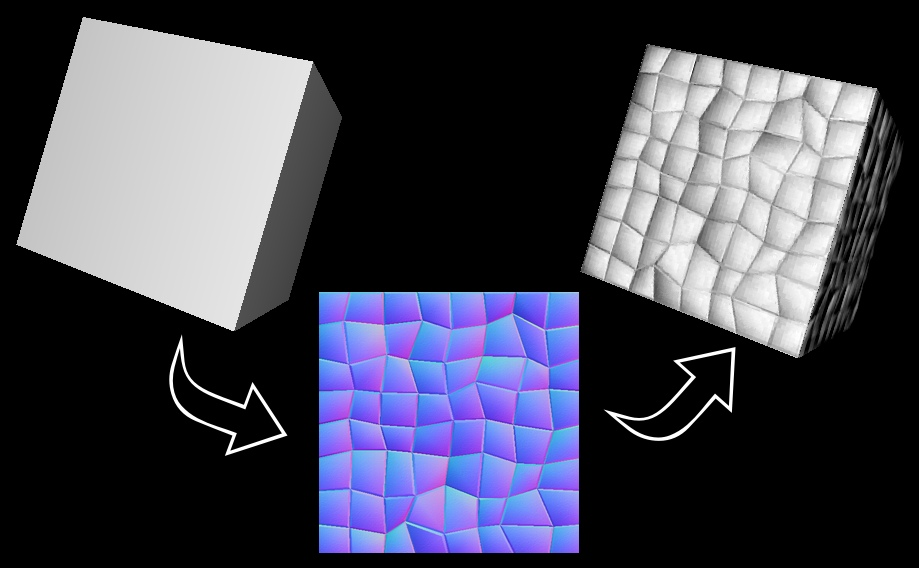
\includegraphics[scale=0.30]{normal_mapping.jpg}
\caption{Illustration de l'effet du normal mapping}
\end{figure}

L’utilisation de ce shader a nécessité la réunification des textures des modèles.
Pour ce faire, Marc a dû fusionner tous les meshes de chaque modèle pour modifier l’UV mapping, puis réunir les textures en une seule en suivant la carte UV.

Ensuite est arrivé l’étape de création des normal map. La technique utilisé habituellement consiste a réalisé deux modèles. Un dit low poly (composé de peu de polygones) et un dit high poly (composé de beaucoup de polygones).

\begin{figure}[htbp]
\centering
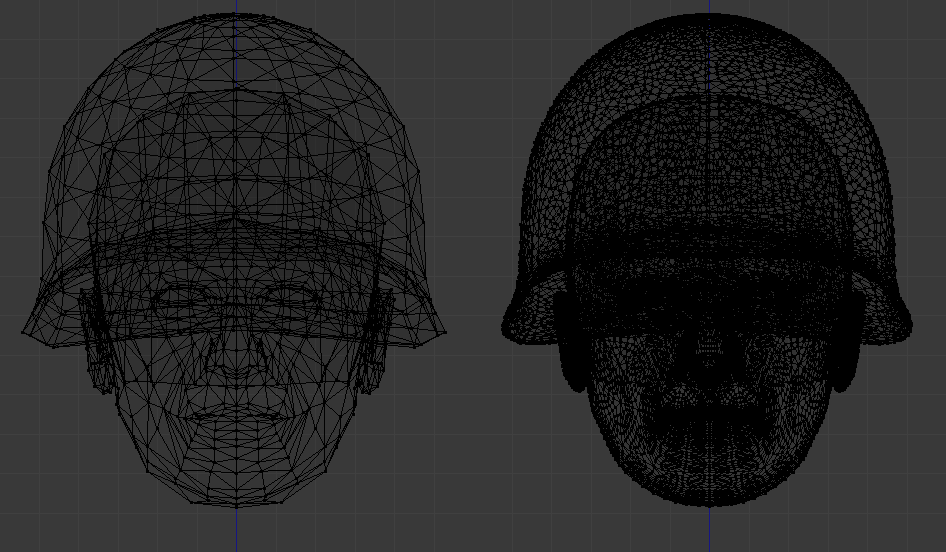
\includegraphics[scale=0.22]{lowpoly_vs_highpoly.png}
\caption{Un mesh en low poly puis en high poly}
\end{figure}

Ensuite on superpose les deux modèles puis le logiciel de modélisation est capable de générer une normal map en calculant la différence de relief en chaque point entre les deux modèles.
Cette technique offre une normal map de qualité, mais est relativement longue puisqu'il est nécessaire de réaliser deux modèles dont un très détaillé.

Heureusement, il existe une autre solution. A partir d'une texture il est possible grâce à un logiciel de retouche d'image, de générer en fonction des couleurs et de la luminosité, une normal map.
Cette technique permet de réaliser rapidement une normal map si la texture de l'objet a déjà été réalisée, et les résultats sont plutôt convaincants. Nous avons donc opté pour la deuxième technique, moins chronophage.

\noindent\textbf{N.B.} Une autre technique permet l'illusion de relief et utilise aussi un shader : le Bump mapping. Cependant, l’image utilisé pour le Bump mapping, a l’instar de celle utilisé pour l'heightmap est en noire et blanc. La modification du relief ne s’effectue que sur un axe (la normale a la surface concernée), le rendu est donc moins détaillé, c'est pourquoi nous avons opté pour le normal mapping.

\begin{figure}[htbp]
\centering
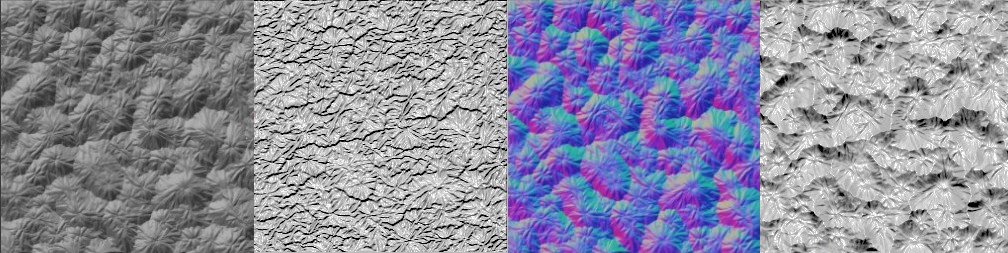
\includegraphics[scale=0.38]{bump_vs_normal.png}
\caption{A gauche le Bump Mapping, à droite le Normal Mapping}
\end{figure}

\subsection{Les animations}

Jusqu'à la première soutenance, les animations 3D n'avait pas fait leurs apparitions dans notre jeu.

Pour cette deuxième soutenance, quelques animations sont visibles. Ainsi le personnages s'accroupit doucement.

Pour obtenir les animations, deux techniques sont possibles. Soit réaliser le modèle et ``programmer'' manuellement les mouvements des différents meshes depuis Visual Studio. Soit réaliser les animations depuis blender et les exportés pour les ``lire'' ensuite.

Par commodité Marc a choisi d’utilisé la seconde méthode. La création d’une animation en utilisant des ``bones''  s’effectue en trois étapes : le ``rigging'', le ``skinning'', et enfin l’enregistrement de l’animation.

Tout d’abord, pourquoi utiliser une armature composée de ``bones'' ?  Cela permet d’animer des modèles complexes, le personnage par exemple, en modifiant le maillage en fonction du mouvement.

\subsubsection{Première étape : le ``rigging''}

Le rigging consiste à créer une armature, un squelette, et à organiser une hiérarchie entre les os.
Il s’agit de disposer les os de façon à être capable d’effectuer les mouvements désirés et d’indiquer la dépendance des os entre eux.

\begin{figure}[htbp]
\centering
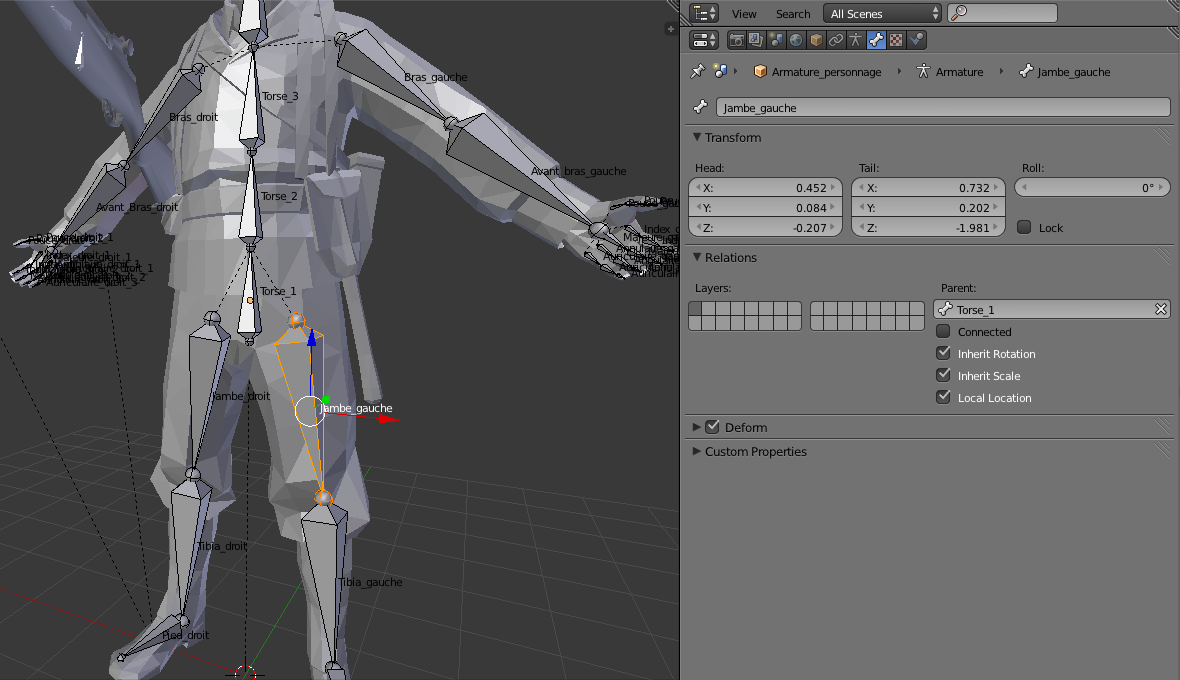
\includegraphics[scale=0.30]{rigging.png}
\caption{Illustration du ``rigging''}
\end{figure}

Un os peut avoir un parent ou non, et peut lui-même être père ou non. Si l’os est père d’un autre alors le mouvement du père entraine le mouvement du fils.

\subsubsection{Deuxième étape : le ``skinning''}

Le skinning consiste à affecter à chaque os les points du maillage sur lesquels il aura une influence, c’est la notion de weight (le poids d’influence). La valeur de ce poids est comprise entre 0 et 1, 0 étant l’influence nulle et 1 l’influence maximale.

Blender offre plusieurs possibilités sur ce point :

\begin{itemize}
\item Soit affecter automatiquement les points du maillage aux os en  fonction de leur ``envelope'', c’est à dire leur rayon d’action.
\item Soit affecter automatiquement les points du maillage aux os en  fonction de leur position par rapport aux os.
\item Soit manuellement. Là encore deux solutions sont possibles :
\begin{itemize}
	\item Sélection de points et affectation a un ``vertex group'', comprendre groupe de point influencé par l’os
	\item Selection par ``Weight Painting'', c’est le même principe sauf qu’au lieu de sélectionner les points du maillage, il suffit de ``peindre'' la surface qui dépendra de l’os.
\end{itemize}
\end{itemize}

\begin{figure}[htbp]
\centering
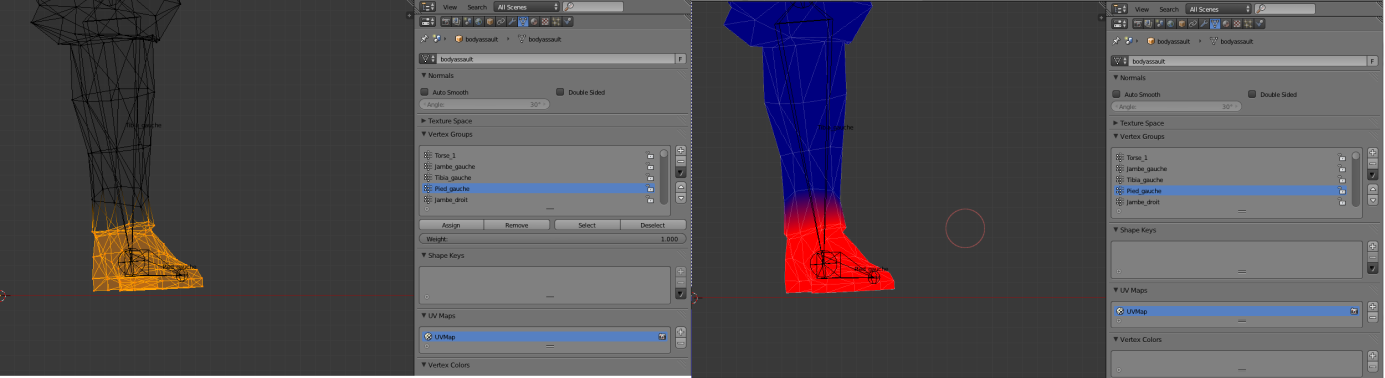
\includegraphics[scale=0.8]{skinning.png}
\caption{Skinning selection maillage à gauche, Weight Painting à droite}
\end{figure}

Les deux premières méthodes de skinning ne sont à utiliser que pour des modeles très simple. Marc n’a donc pas pu les utiliser.

\noindent\textbf{N.B.} Il est très important que tous les points dépendent d’au moins un os. Une solution pour vérifier que tous les points ont un poids et de parcourir les ``vertex groups'' en mode Weight Painting et de chercher une région resté bleue tout le long du parcours.

\subsubsection{Troisième étape : la création de l’animation}

Une fois le squelette construit et les dépendances avec le maillage assignées, il faut maintenant définir les mouvements qui composeront l’animation.

Pour modifier le positionnement des os et que cela ait une influence sur le maillage il faut se placer en ``pose mode''.  Blender permet de diviser l’écran en plusieurs zones pour pouvoir travailler sur différents aspects en même temps. Par défaut sous la vue 3D il y a un zone où le mode ``TimeLine'' est activé. Il s’agit d’un axe représentant le temps sur lequel on peut se déplacer, et servant à indiquer les différents paramètres du modèle en fonction du temps.

C’est grâce a cette ``TimeLine'' que l’on réalise une animation. Il suffit de se placer a un instant t et d’enregistrer les informations voulues pour les liées. Ces instants sont appelées KeyFrames. Ainsi pour l’animation de la cible, à l’instant t1 la cible est relevée, à l’instant t2 la cible est baissée.

Grace à Blender ces deux instants suffisent pour que la cible se baisse et passe de la position-rotation de l’instant t1 a celle de l’instant t2 de manière progressive durant le temps qui sépare ces deux instants. En effet celui-ci va calculer les différents paramètres  à appliquer au modèle à chaque instant pour que l’animation soit fluide.

Une fois l’action créée, il n’y a plus qu’à exporter le modèle.

\subsubsection{Exploitation des animations dans XNA}

Une fois le modèle et l’animation créés et exportés, il va falloir récupérer ces informations pour être capable de lancer l’animation dans XNA. Toutes les informations concernant le modèle sont conservées sous forme de matrice (ex position des points) ou de tableau (ex poids des points, os). 
Par default le ModelProcessor d’XNA pour les fichiers .X ne récupère pas d’information concernant les animations. Il a donc fallu utilisé un autre ContentProcessor pour récupérer les informations de skinning, les  keyframes ainsi que la relation entre les bones.

Pour ce faire nous avons récupérer le sample nommé « Skinned Model » mis à disposition par Microsoft\footnote{\url{http://xbox.create.msdn.com/en-US/education/catalog/sample/skinned_model}}.

Une fois l’extension du Model Processor intégrés à notre code, nous étions en mesure de lancer des animations et de les afficher. Cependant nous nous heurtons à quelques problèmes au niveau de la gestion du temps des animations.

\subsection{Pour la prochaine soutenance}

Pour la soutenance finale, il nous faudra régler nos problèmes de gestion des animations ainsi qu'augmenter l'efficacité du normal mapping. En effet, nous trouvons que la différence n'est pas des plus frappante. Nous essayerons donc d'augmenter l'efficacité du normal mapping.

\newpage
\section{Moteur graphique}

\subsection{La lumières}

Après la première soutenance, nous avons immédiatement homogénéisé la lumière de la scène 3D. Pour cela, nous avons intégré le même calcul de la lumière pour l'ensemble de nos shaders, à savoir : une lumière ambiante, une lumière diffuse et une lumière spéculaire.

\[ I=A_{i}\times A_{c}+D_{i}\times D_{c}\times N\cdot L + S_{i}\times S_{c} \times \left(R\cdot V\right)^{n} \]

Où : \( R=2\times \left(N\cdot L\right)\times N-l \)

\begin{description}
\item[\(A_{i}\)] : Intensité de la lumière ambiante
\item[\(A_{c}\)] : Couleur de la lumière ambiante
\item[\(D_{i}\)] : Intensité de la lumière diffuse
\item[\(D_{c}\)] : Couleur de la lumière diffuse
\item[\(S_{i}\)] : Intensité de la lumière spéculaire
\item[\(S_{c}\)] : Couleur de la lumière spéculaire
\item[\(N\)] : Normale à la surface
\item[\(L\)] : Direction de la lumière
\item[\(R\)] : Vecteur de réflexion
\item[\(V\)] : Position de l'œil
\end{description}

\subsection{Ciel}

L’environnement de notre jeu se composait lors de la première soutenance d’un terrain et de modèle. Nous souhaitions rendre le ciel plus agréable à regarder que la couleur bleue par défaut d’XNA. Notre première idée a été d’utiliser un skydome. Il s’agit d’un modèle 3d prenant la forme d’une demi-sphère sur laquelle est apposé sur la partie intérieure, une image de ciel.

\begin{figure}[htbp]
\centering
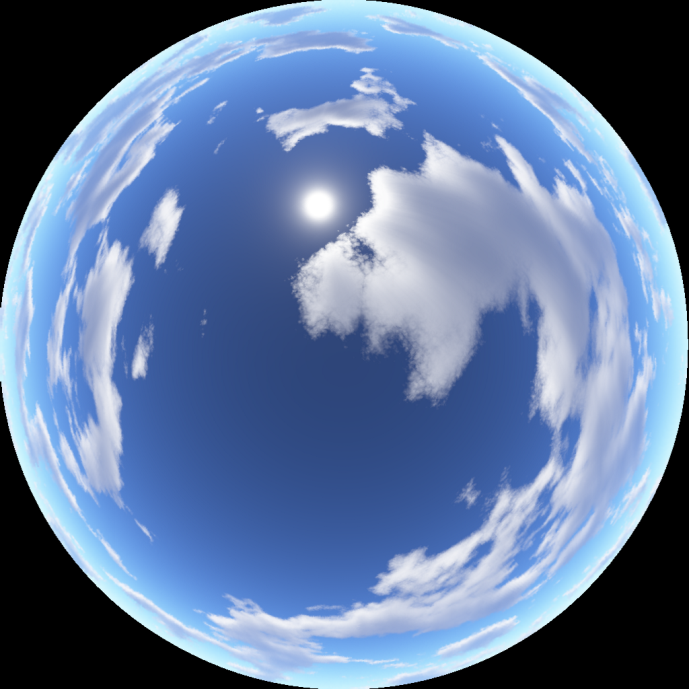
\includegraphics[scale=0.4]{skydome_texture.png}
\caption{Texture d'un skydome}
\end{figure}

Après quelques tests, bien que le rendu soit meilleur qu’un fond bleu uni, nous avons décidé de laisser cette idée de côté.  D’une part parce que la délimitation entre le skydome et le sol posait problème. Et d’autre part car nous trouvions que le ciel restait trop plat !

Nous avons donc fait machine arrière et retiré le skydome. A la place, Thibault a implémenter la gestion de nuage dynamique.

Pour ce faire, il a implémenter une méthode appelé ``Volumetric Clouds''. Cette technique utilise des particules pour donner l'effet de nuage. Les particules sont regroupés par groupe, chaque groupe possède un certain volume de l'espace. Ainsi chaque particules prends une positions aléatoire dans ce volume ce qui permet de rendre différentes sortent de nuages ayant chacun des formes aléatoires.

Une particule est rendu dans l'espace 3D par la technique du billboard. Un billboard est une surface 2D simulant un objet 3D. Le principe du billboard est de toujours faire face à la camera. Ainsi quelques soit l'endroit d'où on regarde, il donnera toujours l'illusion d'être en 3D. L'avantage de cette technique est de réduire la compléxité d'un objet. Ainsi toutes nos particules ne sont qu'un simple triangle.

\begin{figure}[htbp]
\centering
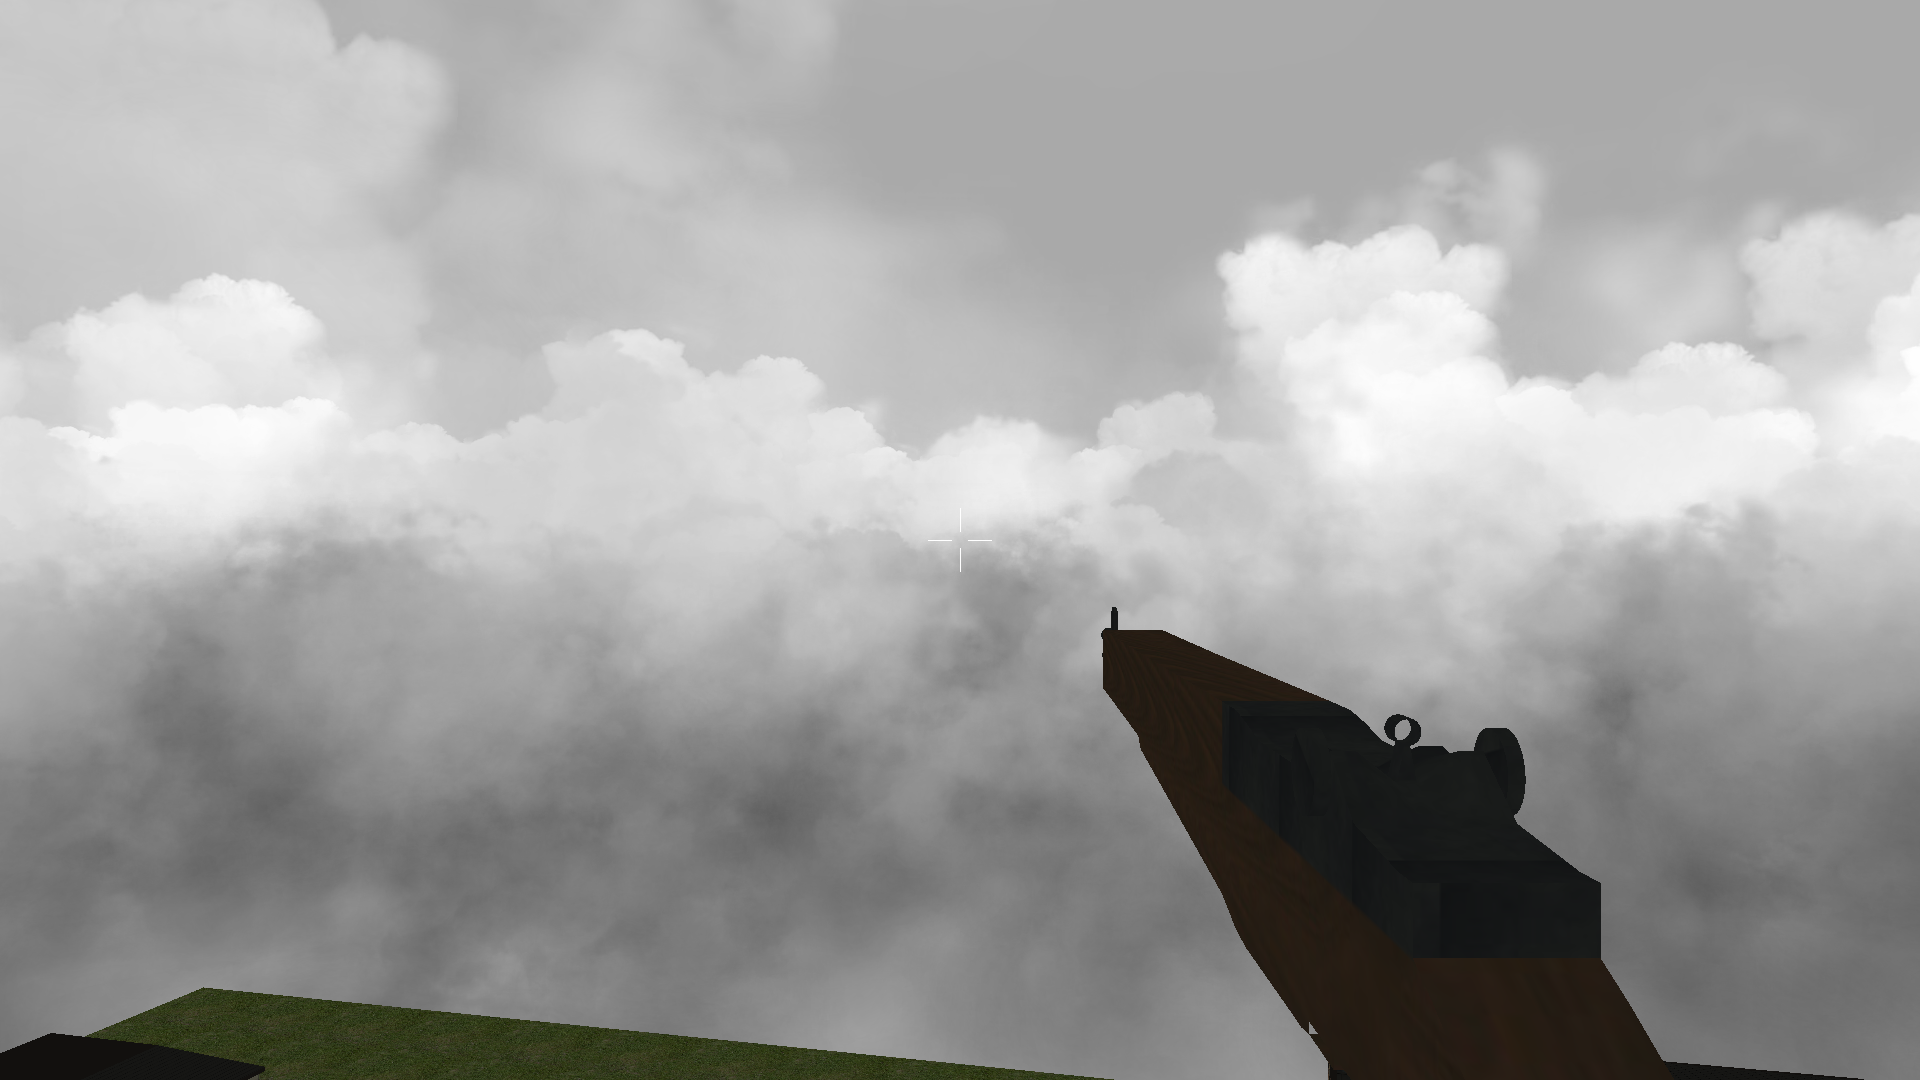
\includegraphics[scale=0.13]{ciel_vue_haut.png}
\caption{Simulation d'un ciel de tempête}
\end{figure}

Mais cela ne suffit pas à avoir des performances correctes. C'est pourquoi Thibault a combiner cette technique avec une autre technique : l'Hardware Instancing, abrégé HI. Il s'agit simplement de rendre plusieurs intances d'un même objet dans une scène en une seule fois. Vue qu'ici nous devons rendre des particules qui sont toutes identiques, cette technique permet de grandement accélérer le rendu.

\begin{figure}[htbp]
\centering
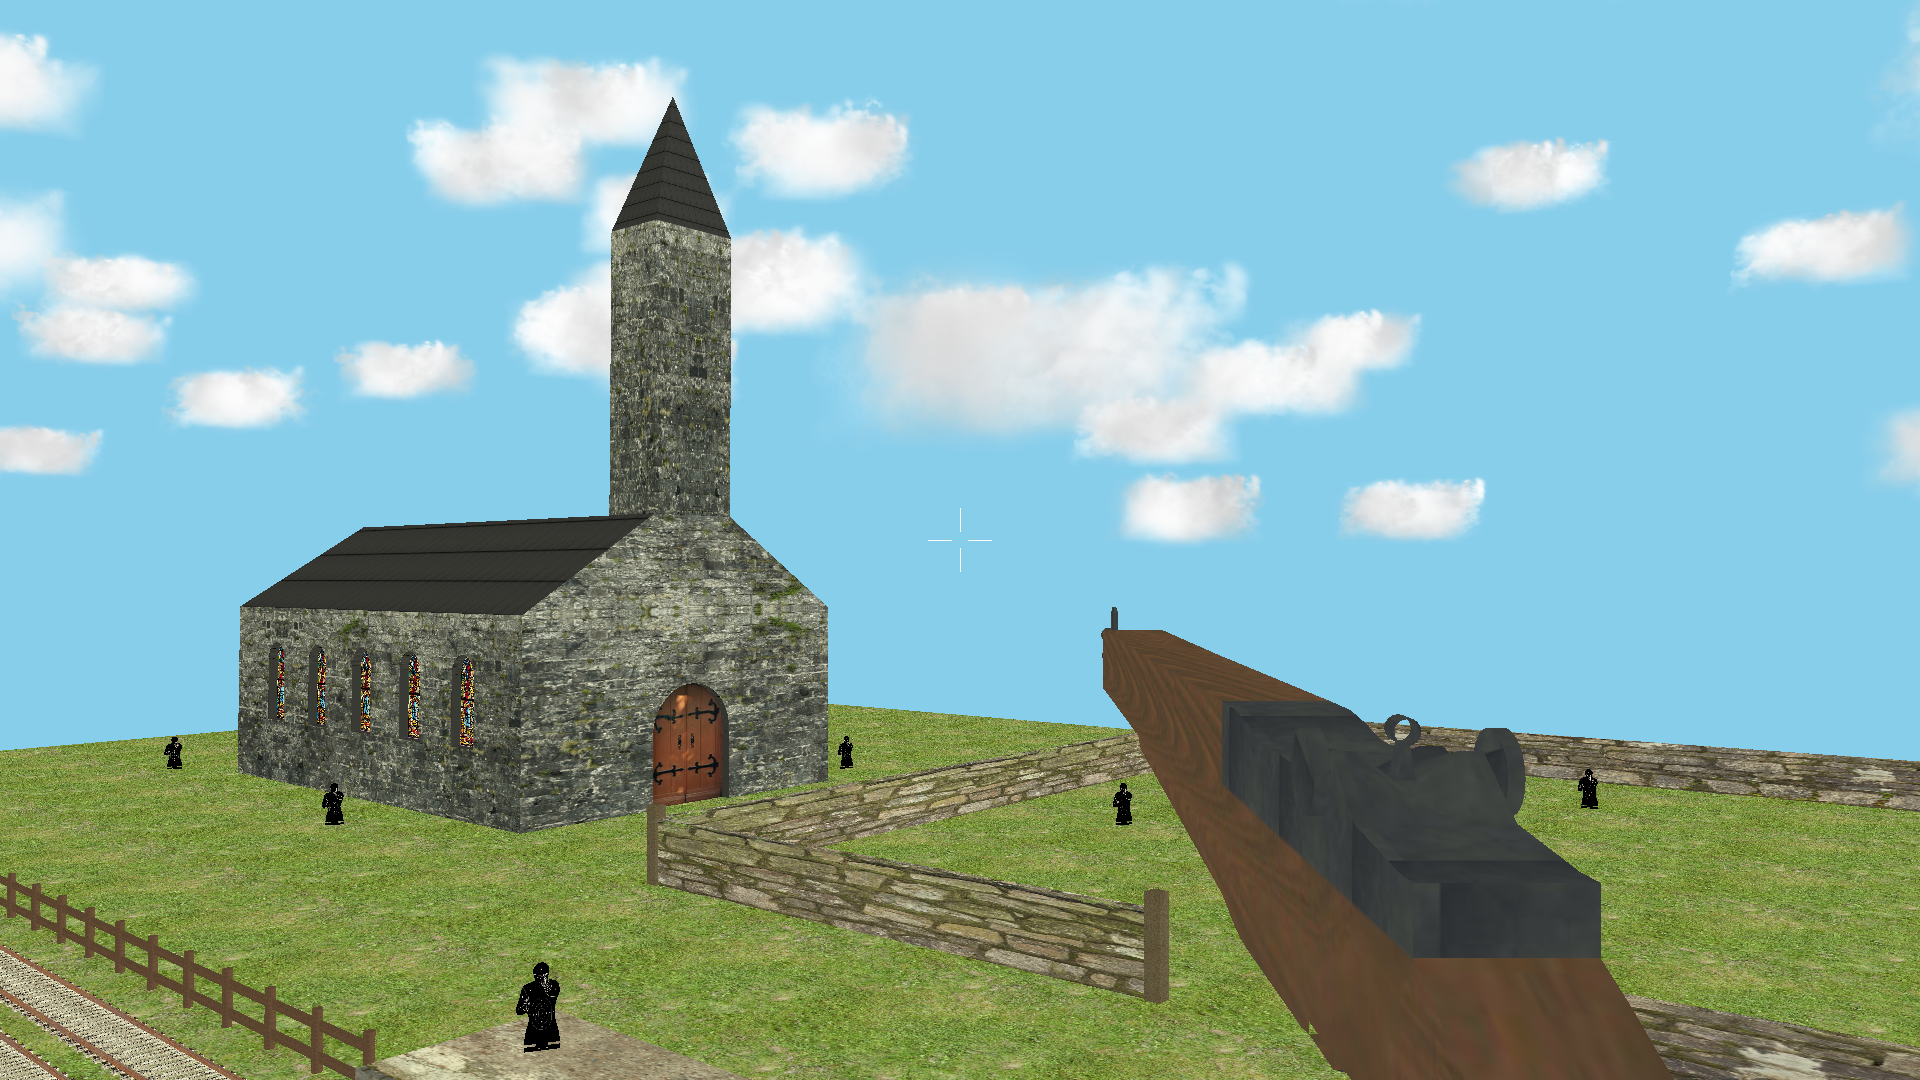
\includegraphics[scale=0.13]{ciel_claire.png}
\caption{Simulation d'un ciel dégagé}
\end{figure}

\subsection{Optimisations}

\subsubsection{Des shaders}

Afin d’optimiser une fois de plus notre moteur de jeu, nous avons réécris nos shaders afin qu’ils soient au maximum compatible avec les preshaders. Les preshaders sont une optimisation du compilateur HLSL qui précalcule les constantes des shaders sur le processeur. Ainsi les calculs utilisant les même valeurs pour l’ensemble des shaders ne sont calculés qu’une seule fois par cycle d'affichage.

Une autre optimisations des shaders a été réalisé au niveau du passage des variables. En effet, le passage de variables au shader implique un transfère des données de la mémoire vive vers la carte graphique. Ce processus fait ralentir les calculs qui doivent attendre le transferts des données. Ce processus est d’autant plus long quand il s’agit de faire passer des textures. Pour contrer ce problème, nous avons décidés de n’actualiser que les données qui varient. Ainsi les textures ne sont transférer au shader que lors de l’initialisation. Nous utilisons donc plus de mémoire graphique mais nos rendus sont grandement accélérés.

\subsubsection{De l'affichage de la map}

Afin de pouvoir afficher de grande map rapidement, nous avons conçu un système utilisant un QuadTree, du Level of Detail, abrégé LOD, ainsi que du Cull Mode.

Le QuadTree est un arbre dont chaque noeud à quatres fils. Il permet de partionner un espace bidimensionnel en le subdivisant récursivement en quatre noeuds. Ici il s'agit de subdiviser le plan \((x,z)\). Ainsi en utilisant un algorithme de Level of Detail, nous sommes capable de changer le niveau de détail de notre map en fonction de la distance qui nous sépare. Enfin, le Cull Mode permet de ``découper'' nos triangles qui compose notre map, pour n'afficher que ceux qui sont visibles. Une fois de plus, cet algorithme tire partie du QuadTree pour optimiser les nombreux tests qu'il génère.

Le but de cette implémentation était de gagner en images affichés par seconde. En effet lors de notre première soutenance, le nombre d'images affichés par seconde était assez faible. Cependant, dans un jeu à la première personne comme le notre, on est très souvent amené à voir la totalité de la map à chaque endroit. De plus il nous faut avoir un vision longue portée. Ainsi, le LOD modifiant à la voler le terrain sous nos yeux rendait le jeu injouable. 

L'option la plus intéressante de cette implémentation restait donc le Cull Mode. Mais il se trouve, qu'après de nombreux tests, notre terrain sans CullMode activé était plus efficace. En effet le Cull Mode nous faisait perdre presque 20 FPS.

C'est pourquoi nous avons préféré optimiser d'autre partie du code (comme l'optimisation des shaders présentés ci-dessus) et revenir sur notre implémentation de base. Nous pouvons aujourd'hui affirmer que c'était la bonne décision étant donné que notre jeu actuelle est moins gourmand au niveau mémoire et processeur que notre première version, alors bien que nous avons un meilleur rendu et des modèles plus lourds.

\subsection{Pour la prochaine soutenance}

Pour la soutenance finale, nous prévoyons diverses améliorations visuelles. Comme par exemple l'affichage des ombres en utilisant la technique du Shadow Mapping.

\newpage
\section{Moteur physique}

Nous avons logiquement décidé d’implémenter un système de collision entre le joueur et les objets de la carte afin de mettre en place un mode solo et multijoueur réaliste.

Cette étape n'a pas été s'en difficulté. Nous nous sommes en effet confronté à divers problème. Tous d'abord la génération des bounding box qui ne fonctionnait pas correctement et puis ensuite la réponse au collision qui n'était pas facile à créer. C'est pourquoi nous avons dès le début implémenter un fonction nous permettant d'afficher les bounding box, afin de nous aider à corriger nos différents bugs.

\begin{figure}[htbp]
\centering
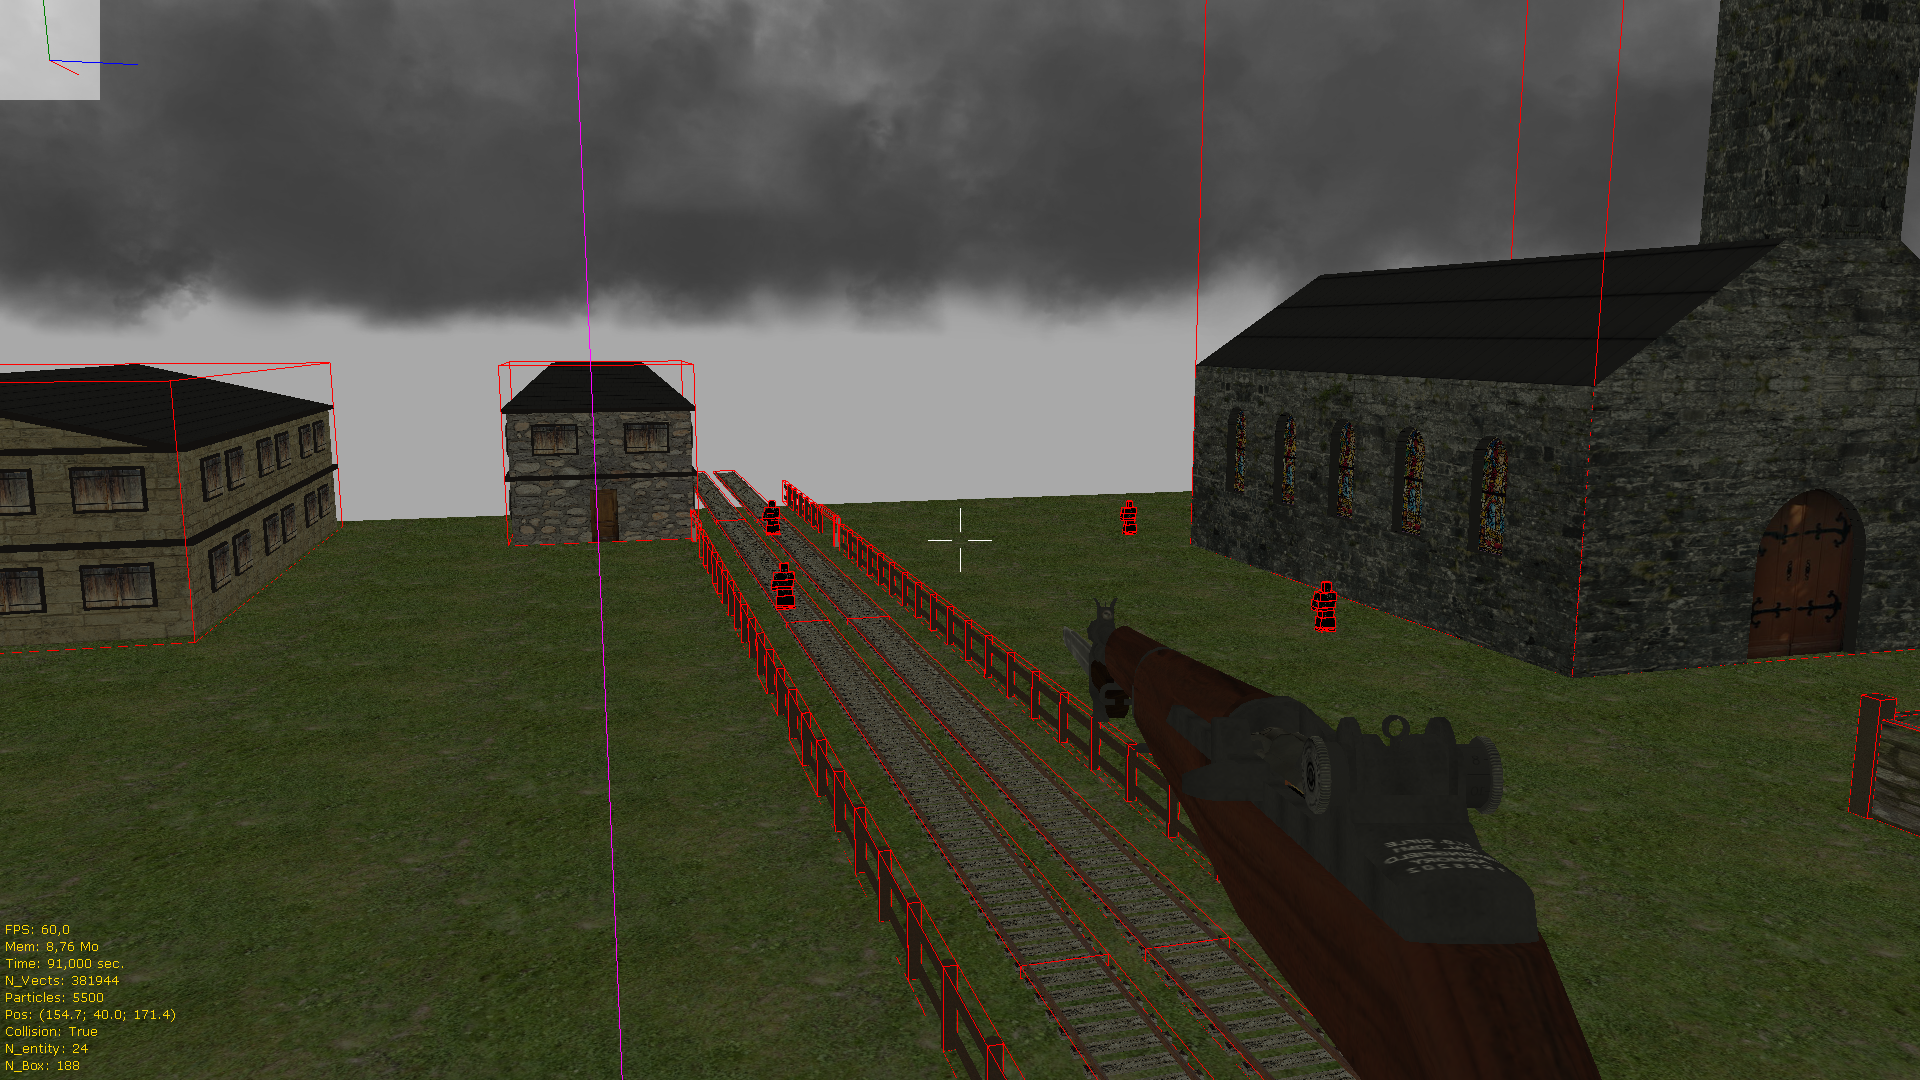
\includegraphics[scale=0.13]{affichage-box.png}
\caption{Affichage des bounding box}
\end{figure}

\subsection{Génération des bounding box}

Afin d'avoir des collisions plus précise, nous avons décidé de générer une bouding box par mesh de chaque objet. Ainsi, pour chaque mesh, notre algorithme parcours son vertex buffer afin d'obtenir les positions de chaque vertices, pour pouvoir trouver le vecteur min et max qui permette de faire construire la bounding box englobant au plus proche la forme du mesh. L'ensemble de ces bounding box sont stocké dans une liste qui nous servira plus tard pour vérifier la présence de collision.

\begin{figure}[htbp]
\centering
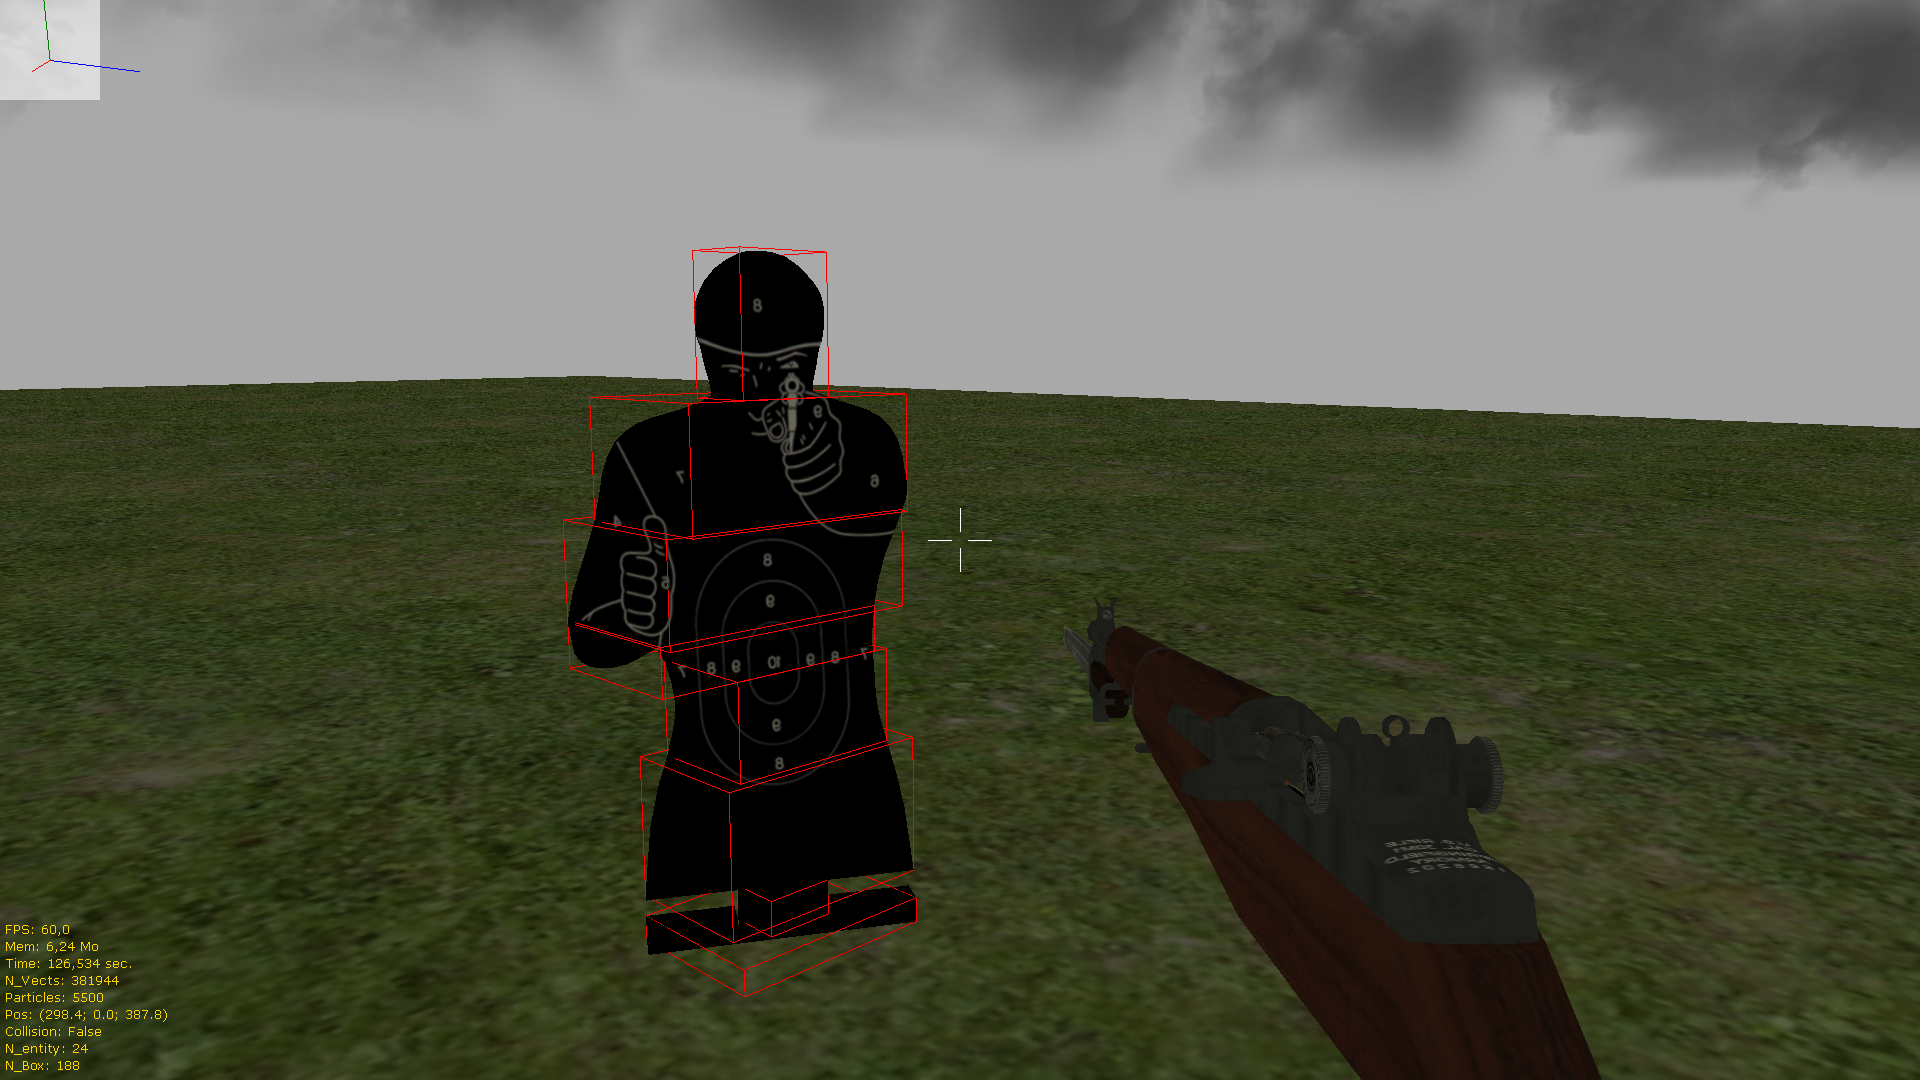
\includegraphics[scale=0.13]{multiple-box.png}
\caption{Bounding box générées pour une cible}
\end{figure}

La génération des bounding box n'est réalisé qu'au chargement d'une partie. En effet l'ensemble de nos modèles sont statique, excepté le joueur qui se déplace.

Pour le joueur, nous avons décidé d'utiliser une bounding sphère, étant donner que la précision est moins importante.

\subsection{Tests des collisions et réponses}

Maintenant que nous avons nos bounding box, nous pouvons à chaque tour de la boucle principale du jeu :

\begin{itemize}
\item Stocker la nouvelle position du joueur dans une autre variable. Il faut garder en mémoire la dernière position du joueur !
\item Générer une nouvelle bounding sphère à la position du joueur calculée précédemment
\item Vérifier si cette bounding sphere rentre en collision avec une des bounding box de la liste
\begin{itemize}
\item Si c'est le cas, il nous faut trouver le point de collision entre la bounding sphère et la bounding box en question. Pour cela, on revient à notre ancienne position et on parcours le vecteur qui relie l'ancienne position avec celle qui à générer la collision (la droite de direction). Une fois ce point obtenu, on peut définir notre position actuelle comme étant le point de collision moins le rayon de la bounding sphère (sur la droite de direction défini plus haut).
\item Si il n'y a pas collision, on peut valider le mouvement et enregistrer la nouvelle position.
\end{itemize}
\end{itemize}

\subsection{Pour la prochaine soutenance}

Pour la soutenance finale, il nous faudra peaufiner notre gestion des collisions. En effet, notre algorithme souffre encore de quelques faiblesses telles que la gestion de collisions multiples et des collisions avec les petits objets.

\newpage
\section{Menu}

\subsection{Écran de démarrage}

Nous avons mis une vidéo au début du jeu qui permet de contrôler l’âge des joueurs qui voudront y jouer pour le rendre plus réaliste. Car, sachant que le jeu est basé sur la guerre, les armes et la destruction pendant la seconde guerre mondiale,  il est préférable d’avertir les utilisateurs du contenu qui va leur être présenté. Ainsi  nous nous sommes mis d’accord que l’âge requis pour y jouer serai de 18 ans.

D’autre vidéos seront bien sûr rajoutées au lancement du jeu tel que l’animation de notre groupe Emagine Studio ou encore une cinématique !

\subsection{Menu principale}

Pour la soutenance 1, nous avions un menu basique avec des boutons et un fond mais il était trop statique, il manquait du mouvement pour qu’il soit plus vivant. Nous avons donc repensé le menu ce qui nous a amené à le refaire entièrement. Le menu est donc devenu dynamique pour cette deuxième soutenance. Un menu composé de boutons repensé, de balles traversant l’écran à des vitesses différentes. Tout un joli paquet de dynamisme qui rend ce menu plus vivant.

De plus nous avons remplacé le bouton jouer par deux boutons qui sont le solo et le multijoueur. 

\begin{figure}[htbp]
\centering
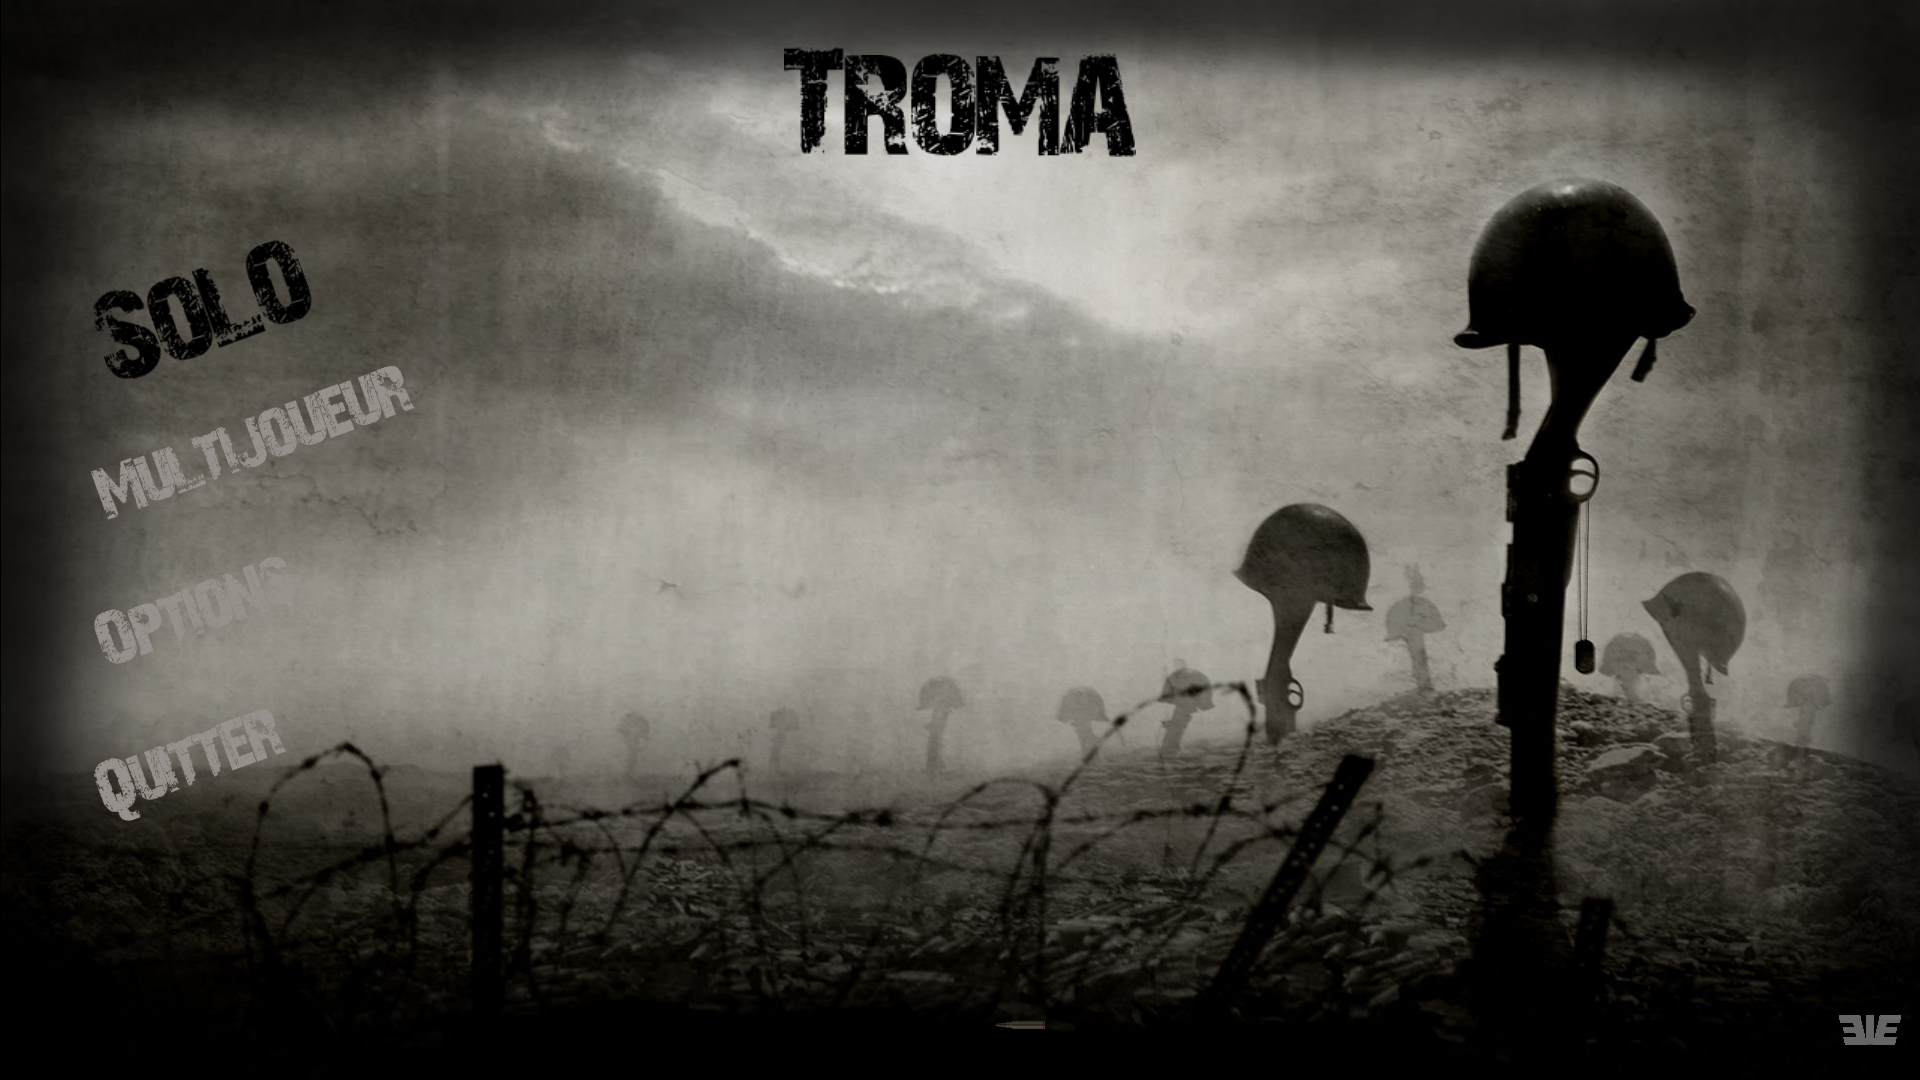
\includegraphics[scale=0.13]{menu-start.png}
\caption{Capture d'écran du menu de démarrage}
\end{figure}

Nous avons aussi ajouté des options. En effet nous avons implémentés des options capables de changer la langue en Anglais ou Français, d’avoir le jeu en pleine écran ou non, de changer le volume du jeu, et de changer le clavier en QWERTY ou AZERTY selon la configuration de touche voulue.

Le joueur pourra ainsi définir ses propres configurations de jeu qui lui permettra de se mettre le plus à l'aise possible et de mieux se plonger dans la peau du personnage.

\begin{figure}[htbp]
\centering
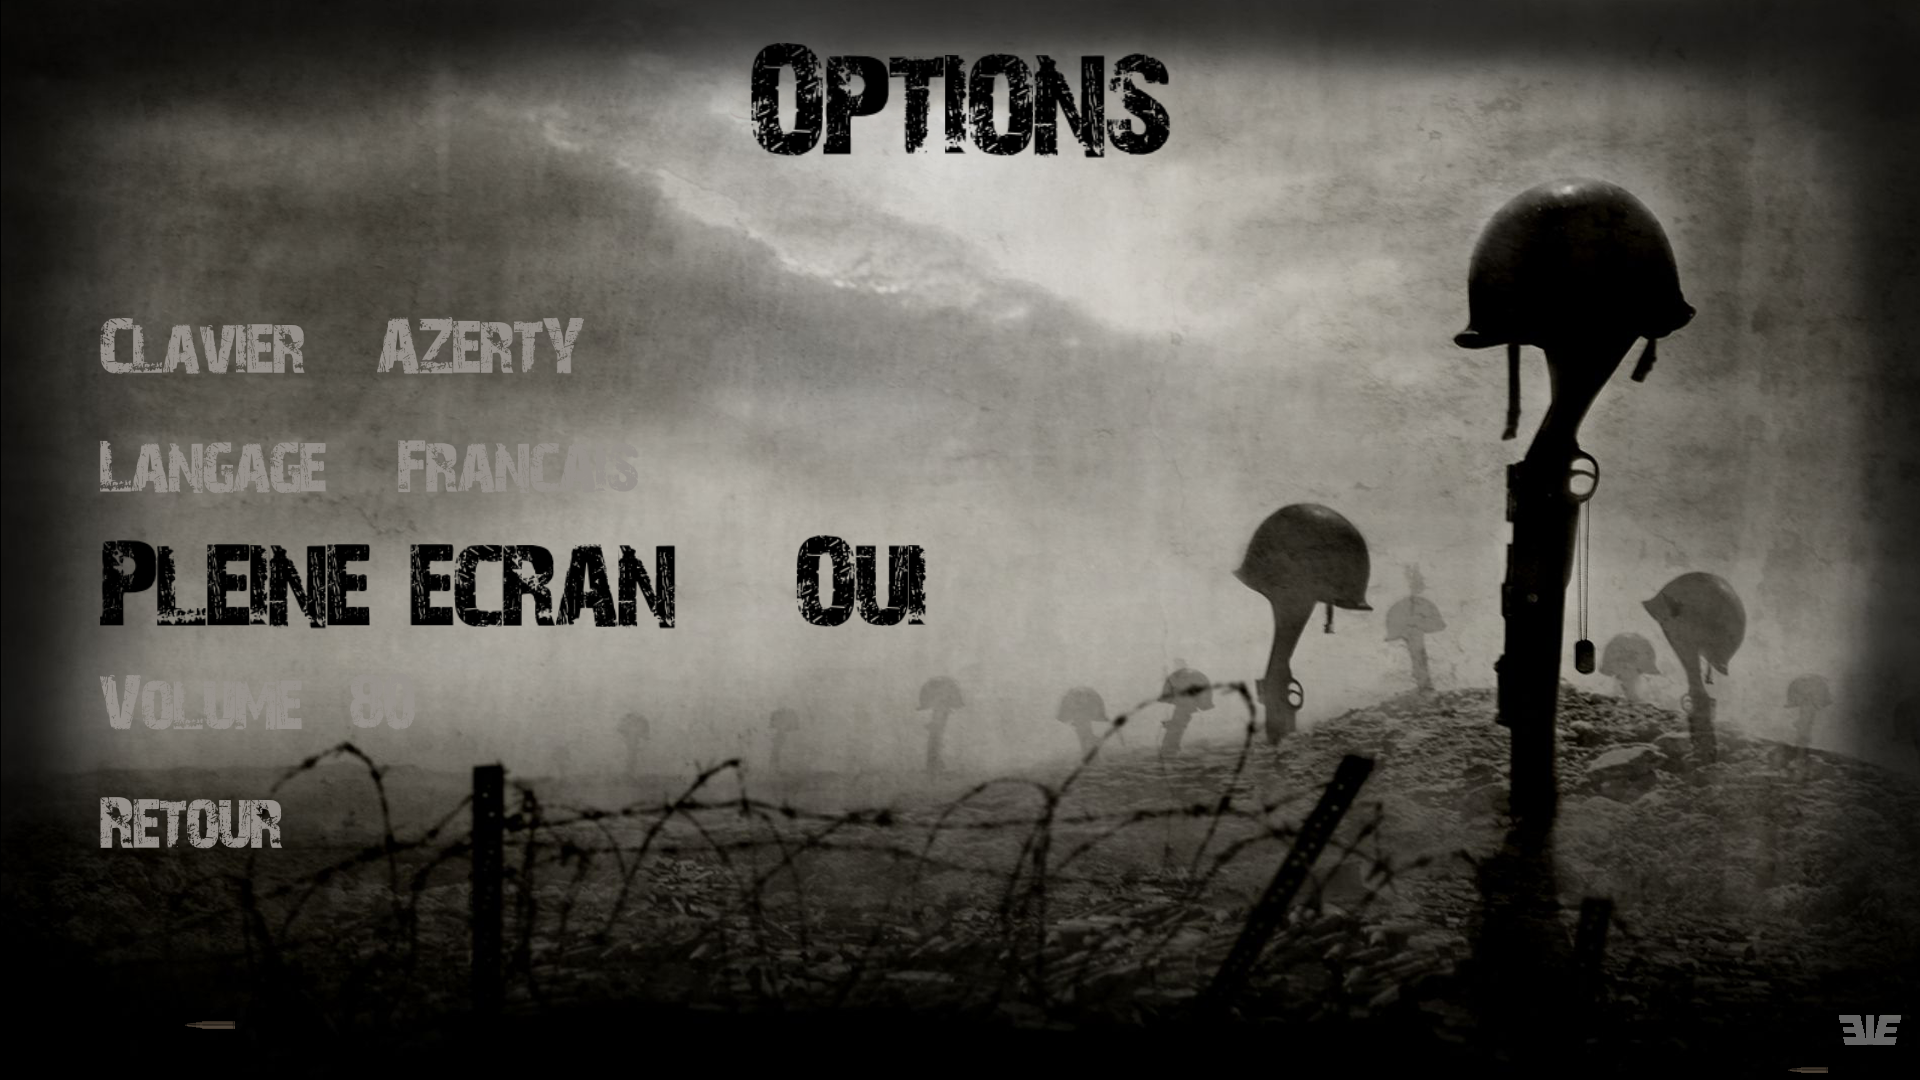
\includegraphics[scale=0.13]{menu-option.png}
\caption{Capture d'écran des options du jeu}
\end{figure}

\subsection{Menu de pause}

Nous n’avons pas tellement évolué le menu de pause. Juste quelque configuration différente telle que le bouton « quitter » qui ramène au menu principal alors qu’avant il quittait directement le jeu. Cela est plus pratique dans le cadre où le joueur voudrait juste changer une configuration dans les options, il pourra donc retourner dans le menu principal au lieu de quitter le jeu. Le seul inconvénient est lorsqu’il relancera le mode solo, sa partie sera remise au début.

Nous pourrons donc rajouter l’accès au menu option directement depuis le menu pause lors de la prochaine soutenance.

\begin{figure}[htbp]
\centering
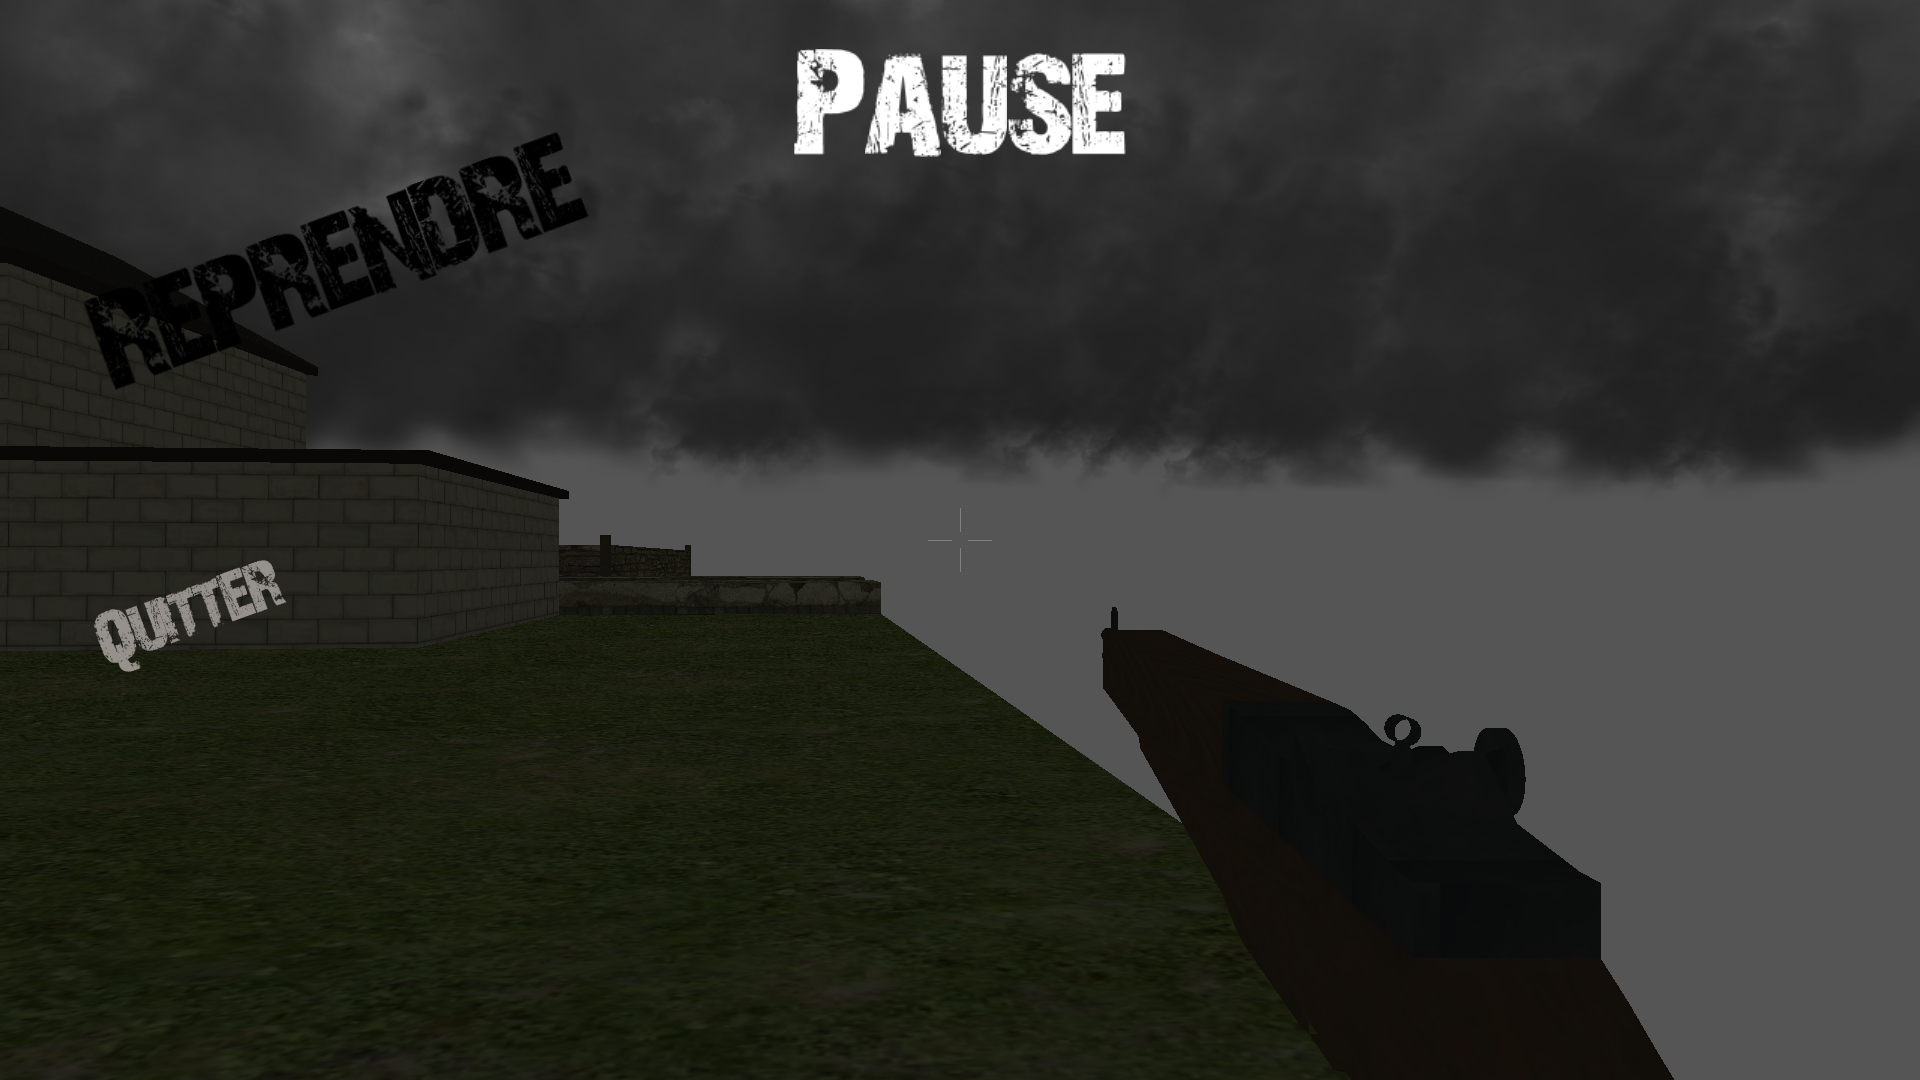
\includegraphics[scale=0.13]{menu-pause.png}
\caption{Capture d'écran du menu de pause}
\end{figure}

\subsection{Pour la prochaine soutenance}

Nous prévoyons d'implémenter le menu multijoueur afin de permettre au joueur de sélectionner une partie. De plus nous implémenterons une page ``Record'' récapitulant toutes les anciennes performances du joueur.


\newpage
\section{Réseau}

Depuis la deuxième soutenance, nous avons commencé l'implémentation du réseau dans notre moteur de jeu. Pour cela, il nous a d'abord fallu réécrire plus de la moitié de notre code pour le rendre compatible avec la logique d'un jeu en réseau.

Une fois cette longue opération fini, nous nous sommes longtemps documenté et nous avons fini par fixer le mode de fonctionnement de notre mode multijoueur. Premièrement, nous avons choisi d'implémenter une architecture client-serveur. 

Le serveur sera chargé de recevoir l'ensemble des entrées de tout les joueurs et faire le calcul de la physique ainsi que de la logique du jeu. Une fois les calculs effectués, le serveur renverra l'ensemble des résultats à l'ensemble des joueurs.

De leur côté, les clients s'occuperont d'envoyer l'ensemble des entrées au joueur ainsi que de faire des calculs de physique approximative. Ainsi le joueur ne devrait pas être gêner par le temps de latence entre lui et le serveur. Les résultat des calculs effectués par le serveur permettront au client de corriger les approximation afin de rester un maximum synchronisé avec le serveur. C'est ce qu'on appelle la technique du ``client side prediction''. Si le client se retrouve totalement désynchroniser par rapport au serveur, par exemple après une perte de paquet trop importante, le serveur utilisera sa temporisation des calculs pour envoyer une commande au joueur avec la position à laquelle il doit se positionner pour être de nouveau synchronisé.

Bien entendu pour réaliser l'ensemble de ces concepts, nous nous baserons sur le protocole UDP, ``user datagram protocol''. Il s'agit d'un protocole de transport de la pile de protocole TCP/IP qui fonctionne sans connexion préalable, par rapport au TCP. Ainsi le protocole UDP ne garantie pas la bonne transmission des données, ni l'ordre d'arrivée. Cependant ce protocole à l'avantage d'être le plus rapide. En effet si un paquet est perdu, le client n'est pas obligé d'attendre que le serveur le renvoi, il recevra directement les paquets suivants. Ainsi il n'y pas de blocage du flux de données par rapport au TCP qui maintient un flux de donnée ordonné dans l'ordre de transmission.

Au niveau de l'implémentation concrète, nous avons choisi d'utiliser la bibliothèque Lidgren\footnote{\url{https://code.google.com/p/lidgren-network-gen3/}}. Il s'agit d'une bibliothèque réseau réputée et conçu en C\#.

Actuellement, nous avons presque fini l'implémentation du client mais nous rencontrons diverses difficultés avec la transmission de données et l'implémentation du serveur. C'est pourquoi le multijoueur n'est pas encore opérationnelle.

\newpage
\section{Gameplay}

A la première soutenance, nous avions un personnage qui était capable de se déplacer dans toute les directions. Celui-ci pouvait tirer mais cela n'avait aucun effet à part émettre un son.

\begin{figure}[htbp]
\centering
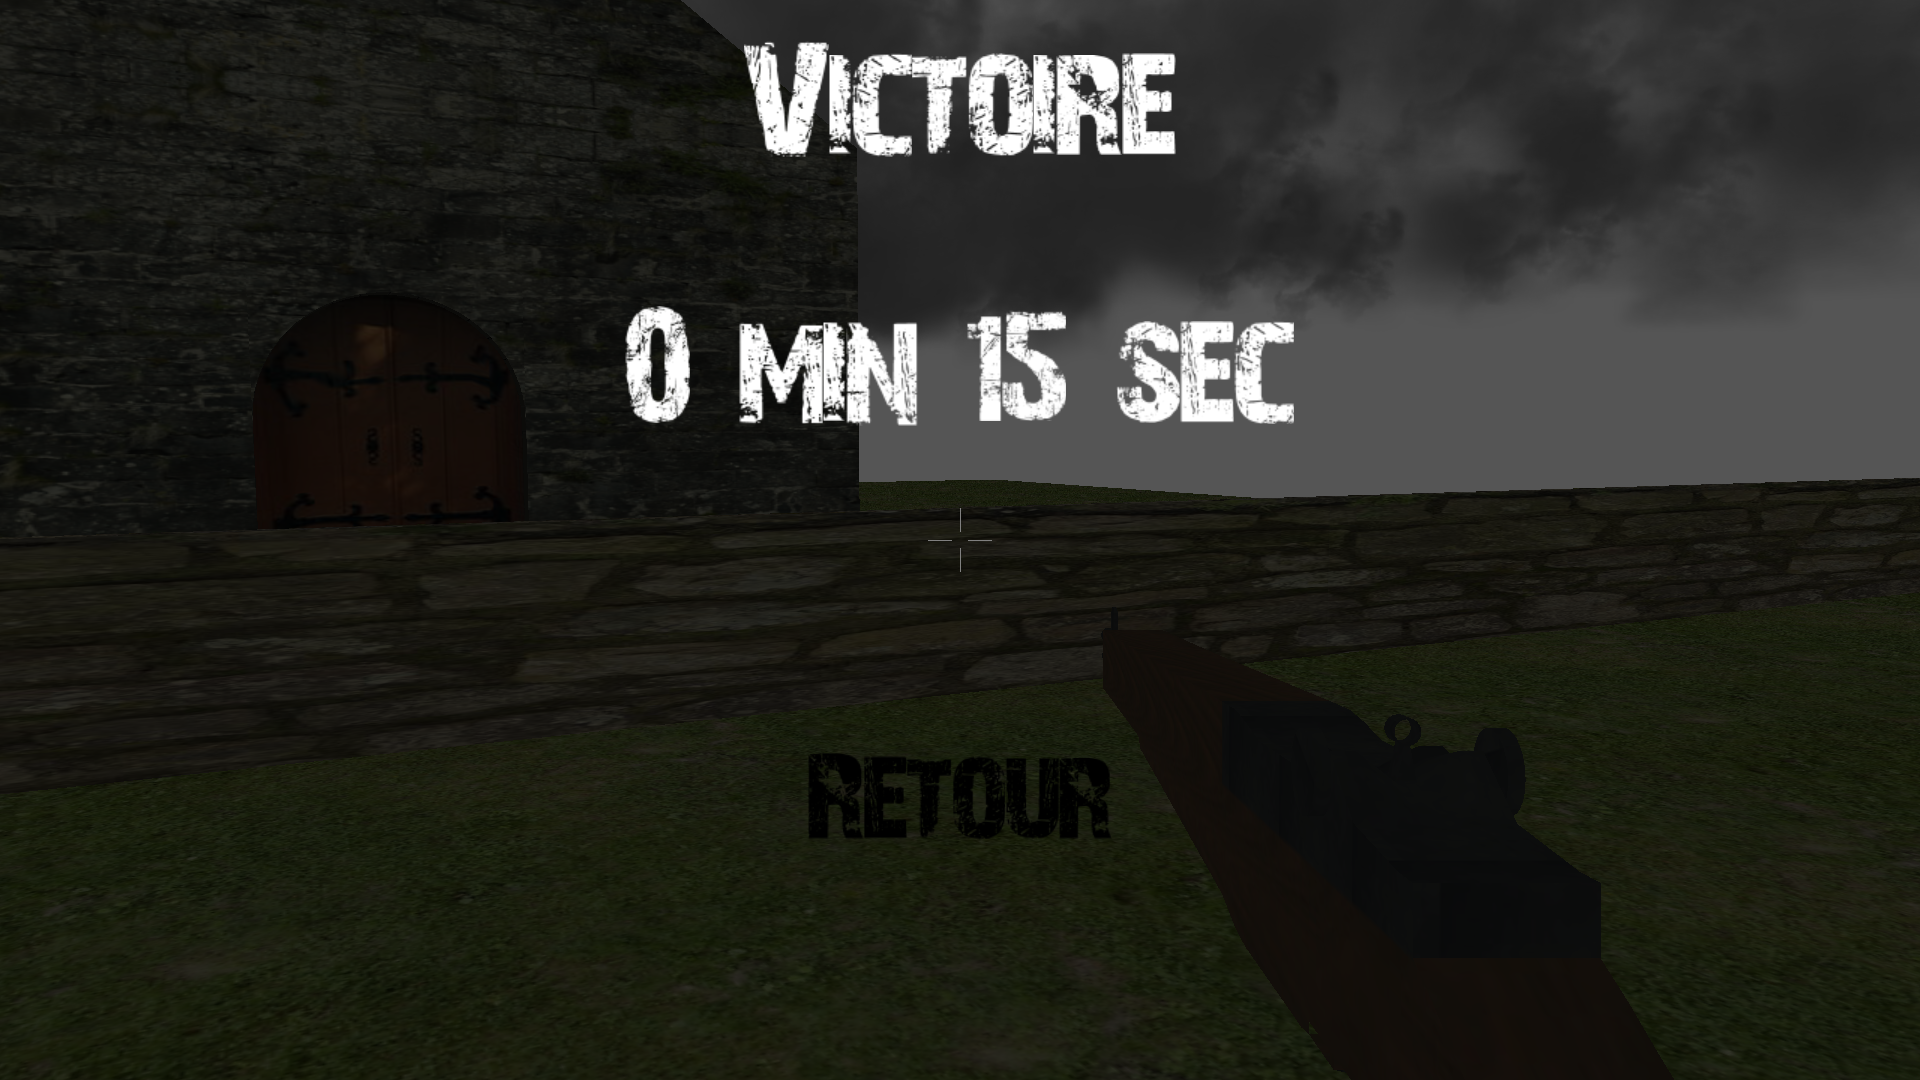
\includegraphics[scale=0.13]{score.png}
\caption{Capture d'écran du score}
\end{figure}

Maintenant que les collisions ont été réalisé, nous avons put intégrer la gestion du tir et des cibles. Ainsi nous avons put réaliser notre mode solo, qui est en réalité principalement un mode d'entrainement pour le mode multijoueur. Dans ce mode, le joueur doit détruire l'ensemble des cibles le plus rapidement possible afin d'avoir le meilleur temps. Ce mode à pour but d'entrainer la réactivé du joueur afin qu'il soit le meilleur dans les futurs parties multijoueurs.

Une fois que toutes les cibles ont été détruites, la partie s'arrête et affiche le temps que le joueur à mis à détruire l'ensemble des cibles. Il en renvient alors à lui même de tenter de battre son record.

\begin{figure}[htbp]
\centering
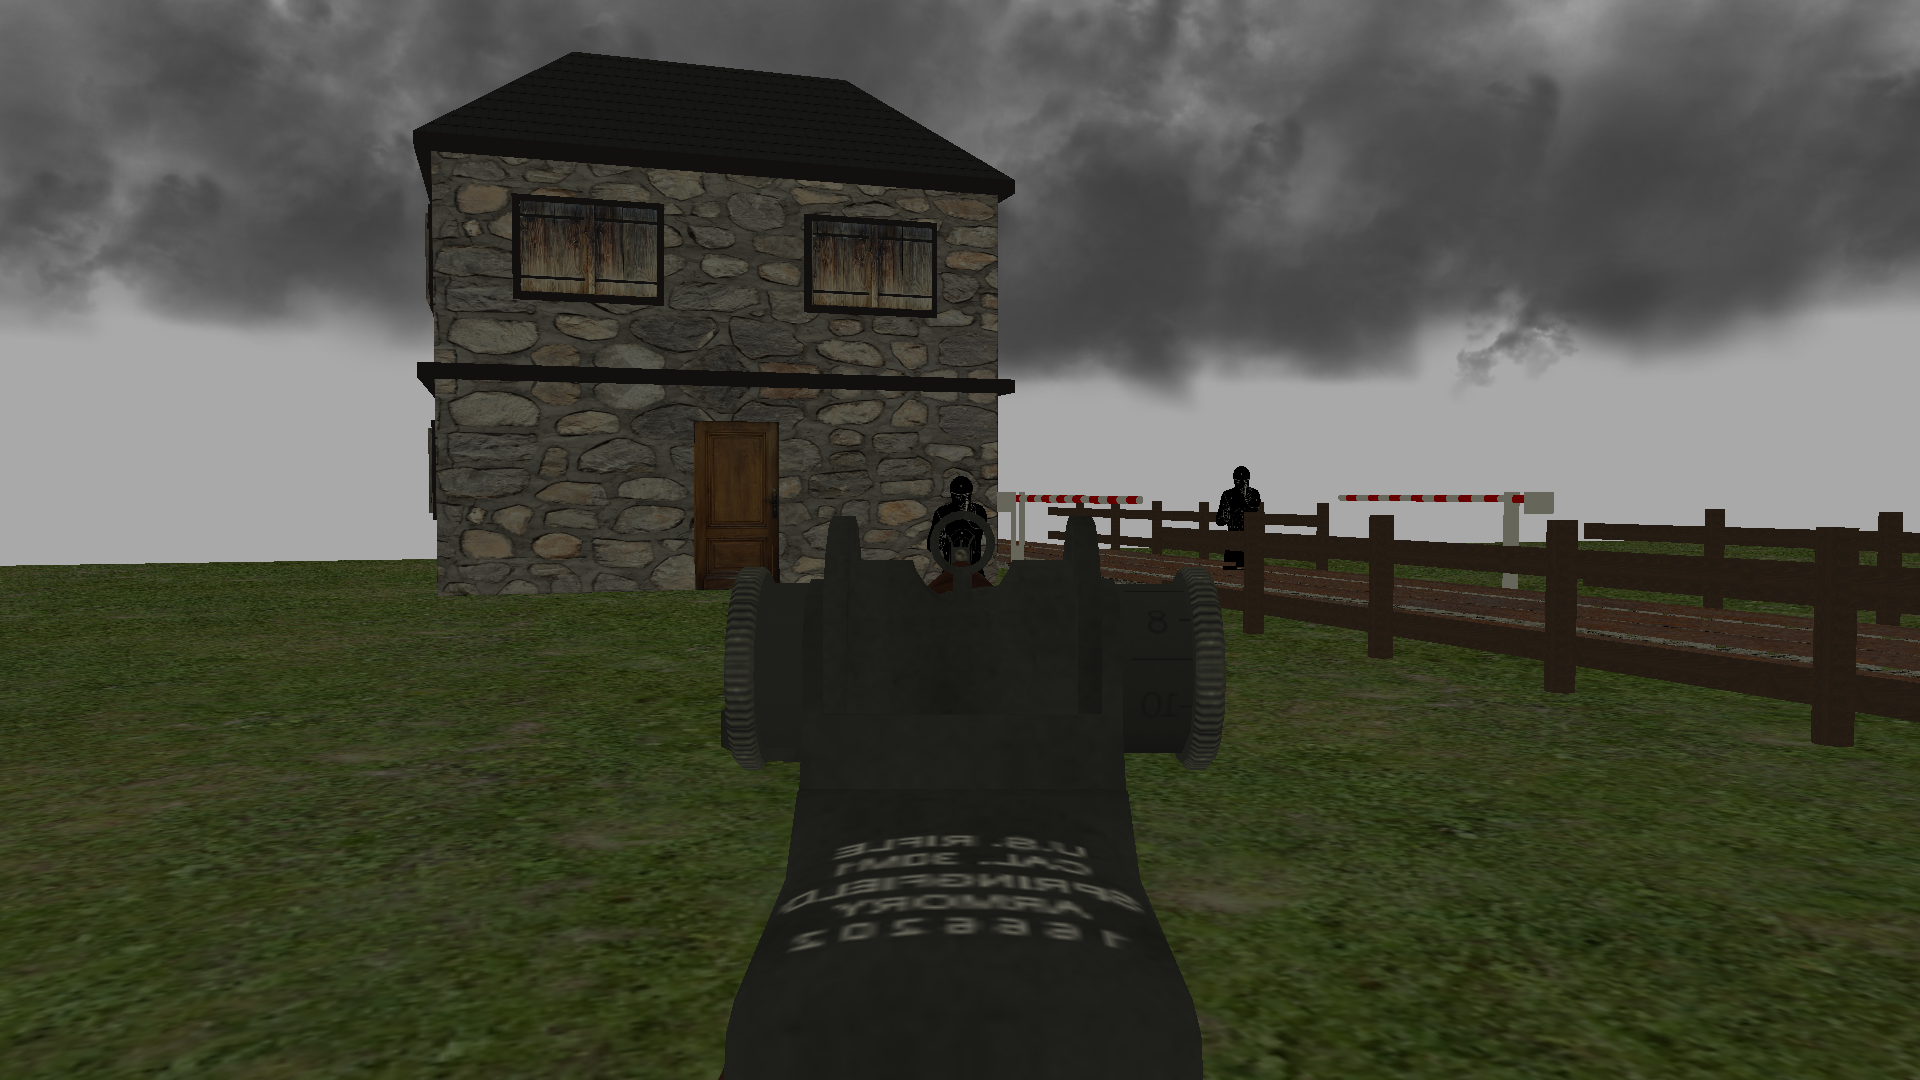
\includegraphics[scale=0.13]{mode-visee.png}
\caption{Capture d'écran du mode visée}
\end{figure}

Avec l'ajout de la gestion du tir, nous avons rajouter un mode visée, permettant une meilleure précision lors des tirs longues distances. De plus il est à noté que nous avons re-modélisé notre arme pour un plus beau rendu.

\subsection{Pour la prochaine soutenance}

Pour l'instant nous avons opté pour une interface des plus minimaliste. Ainsi nous trouvons que l'esprit du jeu qui est d'immerger un maximum le joueur dans la seconde guerre mondiale, est respecté. Mais nous attendons le retour des joueurs de cette nouvelle version pour savoir si l'idée leur plait ou si il préfèrerai une interface leur donnant des informations. Nous nous réservons donc la possibilité de changer l'interface du mode solo.

Mais ce qui occupera un maximum notre temps sera la gestion du gameplay du mode multijoueur.

\newpage
\section{Audio}

Nous avons recodé le gestionnaire du son que ce soit pour la musique dans les menus ou les effets sonores car il ne suffisait plus par rapport au reste du projet.

\subsection{Les effets sonores}

Nous avons rajouté des effets sonores dans les menus pour donner un peu plus de vie dans ceux-ci. Les effets s’appliquent sur les boutons. Quand l’utilisateur utilise les touches directionnelles pour se déplacer entre les boutons, un effet sonore s’applique. De même quand l’utilisateur appuie sur un bouton (par exemple il veut changer la configuration du clavier, quand il va appuyer sur le bouton option, un effet sonore se fera entendre).

Concernant le jeu, nous avons implémenté les bruits de pas pour donner encore plus de réalisme au gamplay. Celui-ci diffère selon l’action, qui est soit de marcher, soit de courir.

Les nouveaux effets sonores ont été pris sur le même site web que les autres qui est \url{http://www.freesound.org/}. Il s’agit d’une banque de sons libre et gratuite.

\subsection{La musique de fond}

Nous avons trouvé une nouvelle musique pour le menu. Celle-ci est une musique de l’époque de la seconde guerre mondiale. Cela permettra au joueur de se mettre tout de suite dans la peau du personnage et dans le style de l’époque.

\newpage
\section{Site web}

Nous avons inclue une section ``actualité'' qui permet de se tenir au courant de l’avancer du projet pour les personnes qui nous suivent. Cette actualité nous sert de petit blog. Nous avons aussi mis à jour le site en changeant les anciennes photos du jeu par les nouvelles. Et nous avons actualisé la partie progression du site internet pour que les internautes voient où l'on se situe par rapport à notre jeu final.\\

\begin{figure}[htbp]
\centering
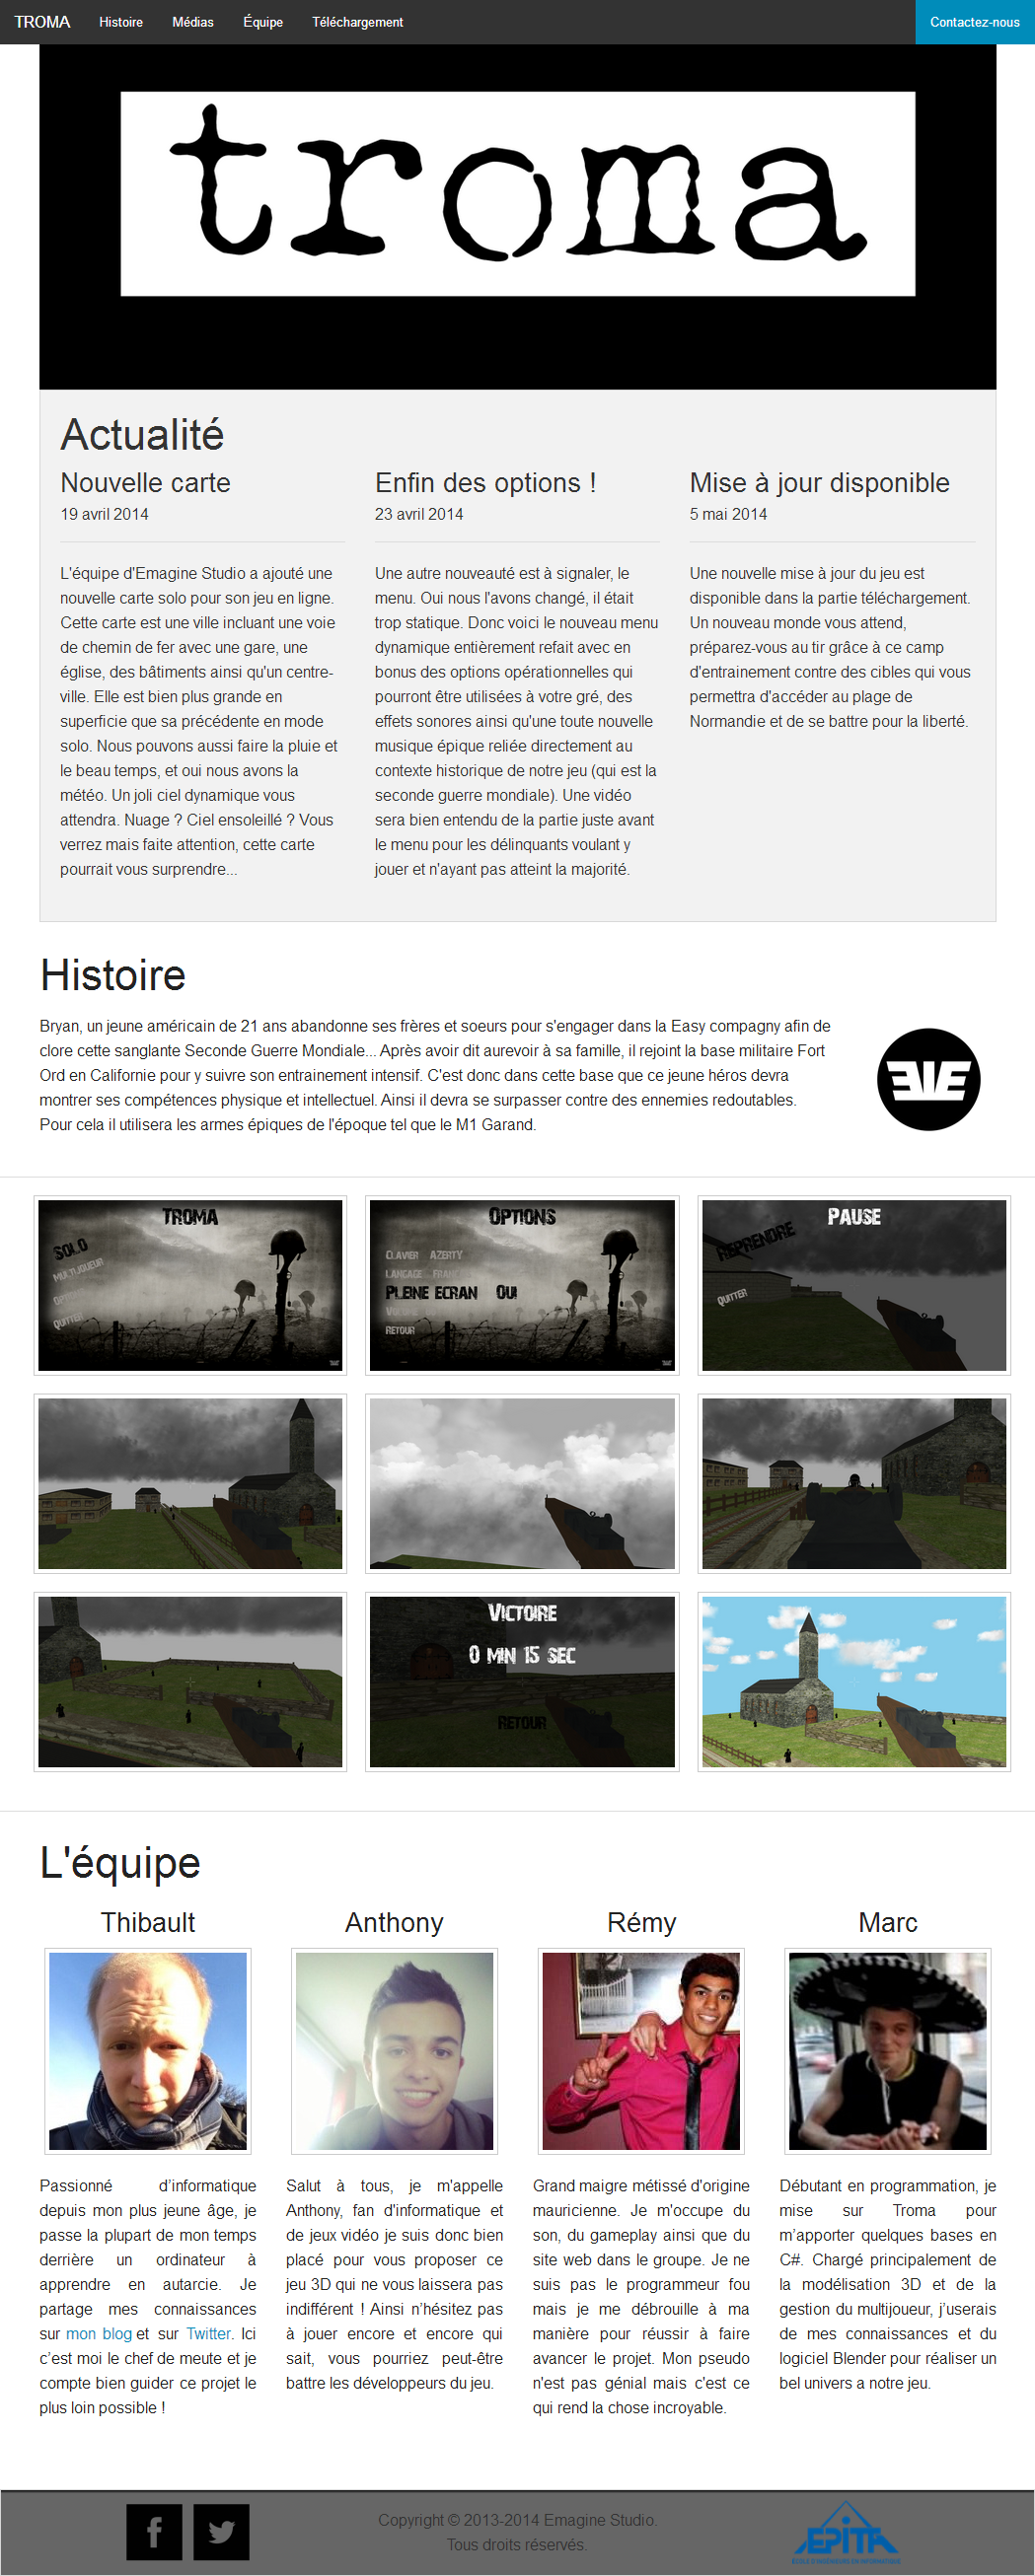
\includegraphics[scale=0.165]{site_web.png}
\caption{Notre site web, le 05/05/14}
\end{figure}

\newpage
\textbf{{\huge Conclusion}} \vspace{7mm}

Cette deuxième période de travail aura été plus difficile. En effet nous avons rencontré de nombreux problèmes. Heureusement nous réussissons toujours à les surmonter à nous quatre. 

Comme expliqué précédemment nous avons pris le temps de recoder la quasi totalité du projet afin de nous préserver de mauvaises surprises quant à l'implémentation du mode multijoueur. De plus, nous avons améliorer ce qui était déjà présent comme par exemple le menu, les sons et autres, en nous servant de nos nouvelles connaissances fraîchement apprises !

Notre projet est d'ores et déjà jouable. Nous allons donc pouvoir nous concentrer pleinement sur le mode multijoueur. Le but étant une nouvelle fois d’améliorer ce que nous avons en y ajoutant en plus tous les éléments prévus pour le rendu final.

Nous souhaitons donc, pour la soutenance finale, vous présenter un jeu complètement fini, sans aucun bug,  et qui propose une expérience de jeu de qualité. Nous voulons que les personnes prennent du plaisir à jouer à notre jeu !\\

\begin{figure}[htbp]
\centering
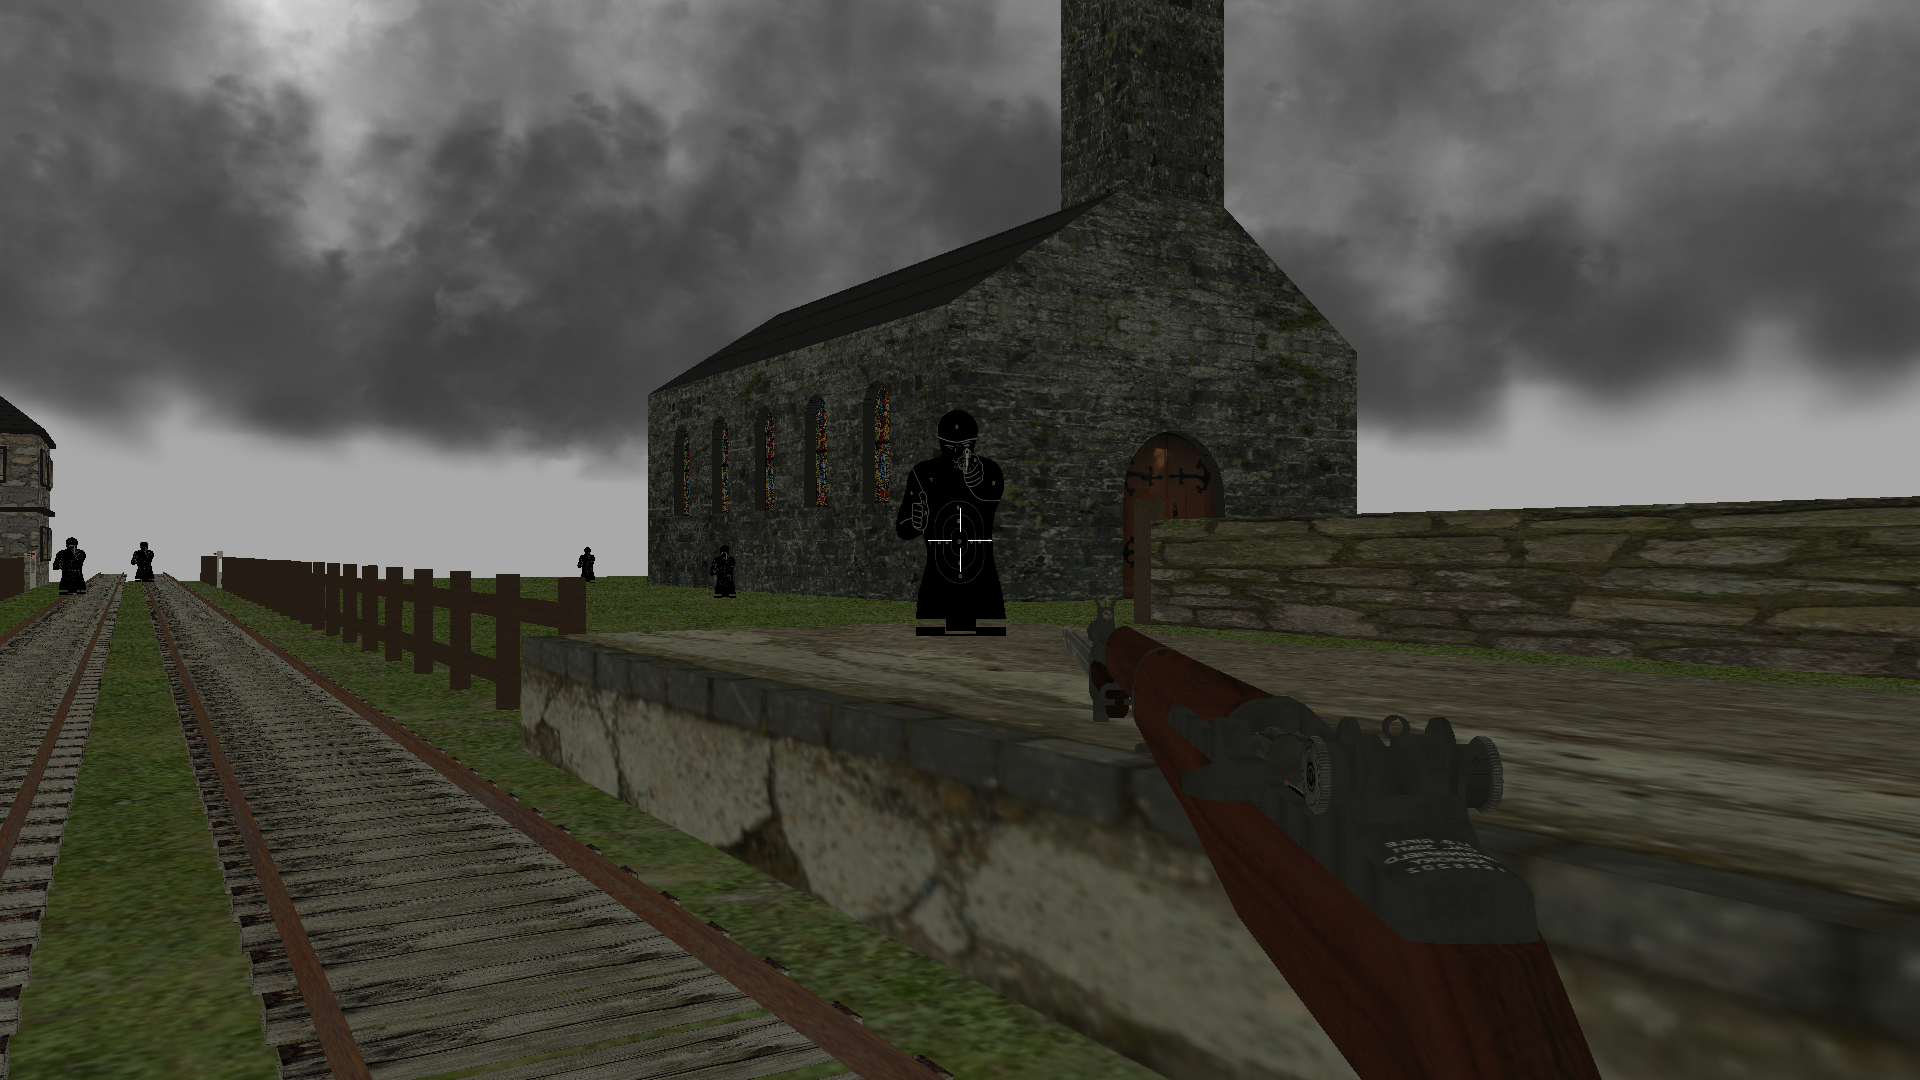
\includegraphics[scale=0.20]{conclu-rendu.png}
\caption{ Capture d’écran du jeu pour la deuxième soutenance}
\end{figure}

\newpage
\listoffigures 
 
\end{document}